\documentclass[12pt]{article}
\usepackage{amsmath, amssymb, amsthm, float, fullpage, graphicx, multirow,parskip, subcaption, setspace}
\usepackage{comment}
\usepackage{url}
\usepackage{tikz}
\usetikzlibrary{shapes.geometric, positioning}
\usetikzlibrary{quotes, angles}
\usepackage{rotating}
\usepackage{hyperref}
\usepackage{natbib}

\definecolor{PennRed}{RGB}{152, 30 50}
\definecolor{PennBlue}{RGB}{0, 44, 119}
\definecolor{PennGreen}{RGB}{94, 179,70}
\definecolor{PennViolet}{RGB}{141, 76, 145}
\definecolor{PennSkyBlue}{RGB}{14, 118, 188}
\definecolor{PennOrange}{RGB}{243, 117, 58}
\definecolor{PennBrightRed}{RGB}{223,82, 78}


\hypersetup{pdfborder = {0 0 0.5 [3 3]}, colorlinks = true, linkcolor = PennBrightRed, citecolor = PennSkyBlue}

\bibliographystyle{apalike}


\newtheorem{theorem}{Theorem}
\newtheorem{acknowledgement}[theorem]{Acknowledgement}
\newtheorem{algorithm}[theorem]{Algorithm}
\newtheorem{axiom}[theorem]{Axiom}
\newtheorem{case}[theorem]{Case}
\newtheorem{claim}[theorem]{Claim}
\newtheorem{conclusion}[theorem]{Conclusion}
\newtheorem{condition}[theorem]{Condition}
\newtheorem{conjecture}[theorem]{Conjecture}
\newtheorem{corollary}[theorem]{Corollary}
\newtheorem{criterion}[theorem]{Criterion}
\newtheorem{definition}[theorem]{Definition}
\newtheorem{example}[theorem]{Example}
\newtheorem{exercise}[theorem]{Exercise}
\newtheorem{lemma}[theorem]{Lemma}
\newtheorem{notation}[theorem]{Notation}
\newtheorem{problem}[theorem]{Problem}
\newtheorem{proposition}[theorem]{Proposition}
\newtheorem{remark}[theorem]{Remark}
\newtheorem{solution}[theorem]{Solution}
\newtheorem{summary}[theorem]{Summary}


\DeclareMathOperator*{\argmax}{arg\,max}
\DeclareMathOperator*{\argmin}{arg\,min}

\newcommand\numberthis{\addtocounter{equation}{1}\tag{\theequation}}


\title{Revisiting the Semi-parametric Latent Factor Model with Regression Trees}
\author{Sameer K. Deshpande}

\onehalfspacing

\begin{document}
\maketitle
\def\C{\mathbb{C}}
\def\R{\mathbb{R}}
\def\Q{\mathbb{Q}}
\def\Z{\mathbb{Z}}
%\def\N{\mathbb{N}}
\def\N{\text{N}}
\def\P{\mathbb{P}}
\def\E{\mathbb{E}}
\def\by{\mathbf{y}}
\def\bx{\mathbf{x}}
\def\bz{\mathbf{z}}
\def\bw{\mathbf{w}}
\def\br{\mathbf{r}}
\def\bu{\mathbf{u}}
\def\bY{\mathbf{Y}}
\def\bX{\mathbf{X}}
\def\bf{\mathbf{f}}
\def\bgamma{\boldsymbol{\gamma}}
\def\bSigma{\boldsymbol{\Sigma}}
\def\bsigma{\boldsymbol{\sigma}}
\def\bmu{\boldsymbol{\mu}}

\def\M{\mathcal{M}}
\def\T{\mathcal{T}}
\def\tilT{\tilde{T}}


\section{General Setup}
\label{sec:introduction}


As a motivating example, consider modeling $q$ physiological time series, which may be highly interdependent and which may be irregularly sampled (i.e. at any one time we may not observe realizations from each series).
The main goal is to impute the value of each time series, to forecast each series several steps into the future, and to provide honest uncertainty quantification about these projections.

Formally, suppose we observe triplets of data $(\bx_{1}, \by_{1}, \delta_{1}), \ldots, (\bx_{n}, \by_{n}, \delta_{n})$ where $\bx_{i} \in \R^{p}$ are covariates (possibly time-dependent), $\by_{i} \in \R^{q}$ are the noisy observations from each series, and $\delta_{i} \in \left\{0,1\right\}^{q}$ is a vector of indicators with $\delta_{i,k} = 1$ if and only if $y_{i,k}$ is observed.
For now, we assume that $\delta$ is deterministic.
\textcolor{blue}{[skd]: in the context of medical time series, this assumption is not particularly realistic. To wit, one series may track the results of a particular diagnostic test that is run only if other vital signs are in some critical region. That is, it's not unrealistic to believe that we observe one series based on the values of previous series. We'll return to this issue later}

Independent of $\delta_{i}$, we model for each $i = 1, \ldots, n$ and $k = 1, \ldots, q$ 
$$
y_{i,k} = f_{k}(\bx_{i}) + \sigma_{k}(\bx_{i})\varepsilon_{i,k}
$$
where $\bf = (f_{1}, \ldots, f_{q})$ and $\bsigma = (\sigma_{1}, \ldots, \sigma_{k})$ are unknown vector valued functions of $\bx$ and the $\varepsilon_{i,k}$'s are independent standard normals.
For now, we focus on the homoskedastic case where the residual variances are constant and do not depend on inputs $\bx_{i}$; we will return to the heteroskedastic case later.

We take a Bayesian approach, which amounts to specifying a prior over the functions $\bf$ and $\bsigma$ and updating them with Bayes' theorem to get posterior distributions that reflect our uncertainty about them in light of the data.
In principle, we can attempt to learn each $f_{k}$ independently of one another in an embarrassingly parallel manner.
This, of course, precludes ``sharing of statistical strength'' and we can quite reasonably expect better predictive performance if we take advantage of the potential correlations between the outcomes \citep[see, e.g.,][]{Breiman1997}. 
Improving prediction of one outcome dimension using information from some or all of the other outcome dimensions has been well-studied in machine learning community, under the name of ``transfer learning'' or ``multi-task learning.''
We borrow from this literature, and refer to each outcome dimensions as a task below.

This is a growing literature that use multi-task GPs regression to model multiple physiological time series (see, e,g., \citet{Clifton2012}, \citet{Ghassemi2015}, \citet{Durichen2015}, \citet{Futoma2017}, \citet{Colopy2018}, and \citet{Cheng2018}). 
Essentially, all of these papers represent each underlying $f_{k}$ as a linear combination of a latent set of independent univariate basis functions, which are assigned GP priors.
In this note, we revisit the semi-parametric latent factor model (SLFM) of \citet{Teh2005} but construct our latent basis using additive regression trees in the style of \citet{Chipman2010} instead of realizations of GPs. 



\section{Proposed Model}
\label{sec:slfm_bart_model}

\subsection{Brief Review of BART}
\label{sec:bart_review}

\citet{Chipman2010} consider the single task regression problem, modeling $y_{i} = f(\bx_{i}) + \sigma\epsilon_{i}, \epsilon_{i} \sim N(0,1)$ and approximate the unknown function $f$ as a sum of regression trees.
To set our notation, let $T$ denote a binary decision tree partitioning $\R^{p}$ that consists of a collection of interior nodes and $L(T)$ terminal or \textit{leaf} nodes. 
We associate an axis-aligned decision rule of the form $\left\{x_{j} < c \right\}$ or $\left\{x_{j} \geq c \right\}$ to each internal (i.e. non-leaf) node of $T.$
$T$ defines a partition of $\R^{p}$ into $L(T)$ rectangular cells and we let $\ell(\bx,T)$ be the function that returns the index of the cell containing the point $\bx.$
A \textit{regression} tree is a pair $(T,M)$ consisting of a decision tree $T$ and collection $M = \left\{\mu_{1}, \ldots, \mu_{L(T)}\right\}$ of parameters corresponding to each leaf of $T.$
We define the evaluation function $g(\bx; T,M) = \mu_{\ell(\bx,T)}$ which takes as input a point $\bx \in \R^{d}$ and returns the leaf parameters corresponding to the partition cell containing $\bx.$
%An illustration in two-dimensions is shown in Figure~\ref{fig:regression_tree}

At the heart of BART is the approximation
$$
f(\bx) \approx \sum_{t = 1}^{m}{g(\bx; T_{(t)}, M_{(t)})}
$$
and a prior over regression trees $\Pi(T,M).$
By modeling each $(T_{t}, M_{t})$ as \textit{a priori} independent realizations from $\Pi(T,M),$ BART implicitly induces a prior over the space of functions from $\R^{p} \rightarrow \R.$
% Figure shows realizations from 
The regression tree prior $\Pi(T,M)$ consists of two parts, a prior $\Pi(T)$ over the space of decisions trees $T$ and a conditional prior $\Pi(M | T)$ of leaf parameters given the decision tree topology.
Conditional on the decision tree $T,$ the associated leaf parameters are modeled as i.i.d. $N(\mu_{\mu}, \sigma^{2}_{\mu}):$ 
$$
\Pi(M | T) = \prod_{\ell = 1}^{L(T)}N(\mu_{\mu}, \sigma^{2}_{\mu}).
$$

% Rather than explicitly write down $\Pi(T)$, we specify it implicitly with a branching. 

The decision tree prior $\Pi(T)$ corresponds to a branching process and can be described in two parts: the probability that a node at depth $d$ is internal and a distribution over the decision rule at each internal node.
Specifically, the probability that node at depth $d$ is internal is $\alpha(1 + d)^{-\beta}$ and conditional on a node being internal, the splitting rule is picked uniformly from the set of all available splitting rules.
Together, these parts induce a prior over the space of functions $f: \R^{d} \rightarrow \R$ and we will write $f \sim \text{BART}(m, \alpha, \beta, \mu_{\mu}, \sigma_{\mu}).$
\citet{Chipman2010} complete their prior specification by placing a scaled inverse-$\chi^{2}$ prior over the residual variance $\sigma^{2} \sim \frac{\nu\lambda}{\chi^{2}_{\nu}}.$
We will denote the induced prior on $f$ as $f \sim \text{BART}(m, \alpha, \beta, \mu_{\mu}, \sigma^{2}_{\mu}).$ 

Key to the success of BART over a wide variety of applied problems has been the existence of useful \textit{default} choices of the associated hyperparameters.
\citet{Chipman2010} recommended setting $\alpha = 0.95$ and $\beta = 2,$ which essentially regularizes the depth of the decision trees $T_{1}, \ldots, T_{m}$ in the BART ensemble.
Now that the prior marginal distribution of $\bf(\bx)$ is $N(m\mu_{\mu}, m\sigma^{2}_{\mu}).$
Upon centering and scaling the observed outcomes, we would like this prior to assign substantial prior probability to the range of the standardized data.
To this end, \citet{Chipman2010} takes $\mu_{\mu} = 0$ and set 
$$
\sigma_{\mu} = \frac{Y_{\max} - Y_{\min}}{2\kappa\sqrt{m}}
$$
where $Y_{\max}$ and $Y_{\min}$ are the maximum and minimum values of the standardized responses.
With these choices, the extremes of the observed data, $Y_{\max}$ and $Y_{\min}$ are within $2\kappa$ marginal prior standard deviations of $f(\bx)$
\citet{Chipman2010} recommended $\kappa = 2$ as a good default value.
All together, the choices $\alpha = 0.95, \beta = 2, \mu_{\mu} = 0$ and $\sigma_{\mu} = 0.5 \times \kappa^{-1}m^{-1/2}(Y_{\max} - Y_{\min})$ regularize the regression trees in the BART ensembles so that they are not too deep and so that no individual tree accounts for too large a portion of the variation in the observed data. 
Put another way, BART seeks to fit the observed data well using an ensemble of ``weak learners.''
With these default choices in mind, abusing our notation slightly, we will take $f \sim \text{BART}(m, \sigma^{2}_{\mu})$ to be a shorthand for $f \sim \text{BART}(m, 0.95, 2, 0, \sigma^{2}_{\mu}).$


\subsection{Proposed Model}

Throughout, we will assume that the observed data from each task has been centered and scaled to have standard deviation one.
In order to perform this scaling, we will require that we observe at least 2 realizations from each task \textcolor{blue}{[skd]: This is one disadvantage vis-a-vis using GPs}.

In order to induce dependence between the $f_{k}$'s, we follow the basic idea of \citet{Teh2004} and introduce independent latent basis functions $u_{1}, \ldots, u_{D}$ and express each $f_{k}$ as a linear combination of these basis elements:
$$
f_{k}(\bx) = \sum_{d = 1}^{D}{\phi_{k,d}u_{d}(\bx)}.
$$
More compactly, we will write $\bf(\bx) = \Phi\bu(\bx)$ where $\bf(\bx) = (f_{1}(\bx), \ldots, f_{q}(\bx))$ and $\bu(\bx) = (u_{1}(\bx), \ldots, u_{D}(\bx))$ and $\Phi = (\phi_{k,d}) \in \R^{q \times D}$ records how much each task $f_{k}$ depends on the basis element $u_{d}.$
We place independent $\text{BART}(m, \sigma^{2}_{\mu})$ priors on each of the basis elements $u_{1}, \ldots, u_{D}$ so that each task $f_{k}$ is now approximated by a weighted sum of regression trees, which are shared across tasks.
This sharing of regression trees induces \textit{a priori} correlation between the tasks.
To see this, first note that conditional on $\Phi,$
\begin{align*}
\text{Cov}(f_{k}(\bx), f_{k'}(\bx) | \Phi) &= \sum_{d = 1}^{D}{\phi_{k,d}\phi_{k',d}\text{Var}(u_{d}(\bx))} \\
&= m\sigma^{2}_{\mu}\Phi_{k,\cdot}\Phi_{k',\cdot}^{\top}
\end{align*}
where $\Phi_{k,\cdot}$ is the $1 \times D$ $\text{k}^{\text{th}}$ row vector of $\Phi.$

It is worth noting that the first line above holds regardless of the prior placed on the basis elements $u_{1}, \ldots, u_{D},$ while the second line follows directly from the fact that the $u_{d}$'s are iid $\text{BART}(m,\sigma^{2}_{\mu}).$
Now so long as the prior on $\Phi$ assigns positive probability to the event $\Phi_{k,\cdot}^{\top}\Phi_{k',\cdot} \neq 0,$ $f_{k}(\bx)$ and $f_{k'}(\bx)$ will be marginally correlated as well. 

Just like with univariate BART, we aim to set useful default hyperparameter specifications.
To this end, we start with $\sigma_{\mu} = \frac{Y_{\max} - Y_{\min}}{2\kappa \sqrt{mD}}$ where $\kappa$ is to be specified, where $Y_{\max}$ and $Y_{\min}$ are the maximum and minimum standardized observations across all observations.

We place independent scaled inverse-$\chi^{2}$ priors on the residual variances $\sigma^{2}_{1}, \ldots, \sigma^{2}_{q}$, with $\sigma^{2}_{k} \sim \text{Inv. Gamma}\left(\frac{\nu}{2}, \frac{\nu\lambda_{k}}{2}\right).$
We use \citet{Chipman2010}'s default choice of $\nu = 3$ and pick $\lambda_{k}$ so that \textit{a priori} $\P(\sigma_{k} < \hat{\sigma_{k}}) = 0.9$ where $\hat{\sigma}_{k}$ is an initial over-estimate of the residual standard deviation for task $k.$
That is, we take $\lambda_{k} = \nu^{-1}q_{\nu,0.1}\hat{\sigma}^{2}$ where $q_{\nu,0.1}$ is the 10\% quantile of the $\chi^{2}_{\nu}$ distribution.
For $\nu = 3$ and $\hat{\sigma}_{k} = 1$, which is a reasonable over-estimate of the residual variance once we standardize all responses, we have $\lambda_{k} \approx 0.195.$


It remains to specify the prior on $\Phi$ and to set the number of basis elements $D$ and the number of trees within each basis element $m.$
Recall that one of the key feature of univariate BART is the fact that the marginal prior on $f(\bx)$ gave substantially probability to the range of the observed responses.
While this type of calibration does sacrifice Bayesian coherence, it does ensure that the prior on $f$ is not grossly in conflict with the data.
To achieve a similar calibration, notice that conditional on $\Phi$, 
$$
\bf(\bx) | \Phi \sim N_{q}(0_{q}, m\sigma^{2}_{\mu}\Phi\Phi^{\top}).
$$

One way to ensure that the marginal prior on $f_{k}$ covers the range of observed realizations of the $\text{k}^{\text{th}}$ task is to require 
$$
\sqrt{m}\sigma_{\mu}\lVert \Phi_{k,\cdot}\rVert_{2} \ll Y_{k,\max} - Y_{k,\min}
$$
with high prior probability.
Recalling our choice of $\sigma_{\mu} = \frac{Y_{\max} - Y_{\min}}{2\kappa \sqrt{mD}}$, we can achieve this desideratum if 
\begin{equation}
\label{eq:phi_desideratum}
\lVert \Phi_{k,\cdot} \rVert_{2} \leq \sqrt{D} \times \frac{Y_{k,\max} - Y_{k,\min}}{Y_{\max} - Y_{\min}},
\end{equation}
with high prior probability.


As a starting point, consider the relatively simply prior $\phi_{k,d} \sim N(0, \sigma^{2}_{\phi,k}).$
With this choice, we note that $\lVert \Phi_{k,\cdot} \rVert_{2}^{2} \sim \sigma^{2}_{\phi,k}\chi^{2}_{D},$ so one way to achieve~\eqref{eq:phi_desideratum} \textit{marginally} for each $k = 1, \ldots, q$ is to set
$$
\sigma_{\phi,k} = \left(\frac{D}{q_{D,0.9}}\right)^{1/2} \times \frac{Y_{k,\max} - Y_{k,\,min}}{Y_{\max} - Y_{\min}}
$$
where $q_{D,0.9}$ is the 90\% quantile of a $\chi^{2}_{D}$ distribution.
Note that we can easily use a different quantile.

A slightly stronger requirement may be to satisfy~\eqref{eq:phi_desideratum} simultaneously for each task, which motivates taking
$$
\sigma_{\phi,k} = \left(\frac{D}{q_{D,0.9^{1/q}}}\right)^{1/2}\times \frac{Y_{k,\max} - Y_{k,\min}}{Y_{\max} - Y_{\min}}.
$$

It is worth pointing out that as $D \rightarrow \infty,$ the ratio $\frac{D}{q_{D,\tilde{\alpha}}} \leftrightarrow 1$ for any $\tilde{\alpha} > 0.5$
We note that larger choices of $\sigma^{2}_{\phi,k}$ induce \textit{less} regularization on the fit of $f_{k}$ since it disperses more marginal probability mass of $f_{k}$ outside the interval $[Y_{k,\min}, Y_{k,\max}].$

Note that under this simple prior specification, each task $f_{k}$ depends on every basis function $u_{d},$ and therefore each of the tasks are \textit{a priori} correlated.
In some situations, this may be overly restrictive or unrealistic. 
A more flexible option that can adapt to the situation that some of the tasks are uncorrelated is to use a sparsity inducing prior on the elements of $\Phi.$
\textcolor{blue}{[skd]: Another motivation: the cross-covariances depend on a matrix of rank $\min\left\{D,q\right\}$. We could want adaptivity}
Specifically, we can introduce binary indicators $\gamma_{k,d}$ and model 
\begin{align*}
\phi_{k,d} | \gamma_{k,d} &\sim \gamma_{k,d}N(0,\sigma^{2}_{\phi,k}) + (1 - \gamma_{k,d})\delta_{0} \\
\gamma_{k,1}, \ldots, \gamma_{k,d} | \theta_{k} &\stackrel{\text{i.i.d}}{\sim} \text{Bernoulli}(\theta_{k}) \hspace{0.1in} \text{for $k = 1, \ldots, q$}\\
\theta_{1}, \ldots, \theta_{q} &\sim \text{Beta}(a,b)
\end{align*}

To set an appropriate value of $\sigma^{2}_{\phi,k},$ we note that $\sigma^{-2}_{\phi,k}\lVert \Phi_{k,\cdot} \rVert_{2}^{2}$ is now a $\chi^{2}$ random variable with a \textit{random} number of degrees of freedom equal to the number of non-zero $\phi_{k,d}.$
\textcolor{blue}{[skd]: I'm still thinking about the details but I'm pretty sure the number of non-zero entries concentrates around it's mean and we can probably do something with that.}


\subsection{Connection to Existing Work}
\label{sec:related_work}

Our model is closely related to (and in fact, inspired by) the semi-parametric latent factor (SFLM) of \citet{Teh2004}, who introduce independent basis functions $u_{1}, \ldots, u_{D}$ and loading matrix $\Phi \in \R^{q \times D}$ and model $\bf = \Phi \bu.$
In that work, they place Gaussian process priors on the basis functions, $u_{d} \sim \text{GP}(k_{d})$ while have placed BART priors on them. 
In fact, the SLFM is a special case of the liner model of coregionalization (LMC) that is commonly used for fitting multi-output GPs \citep[see, e.g.][]{Alvarez2012}.
At a high-level, the LMC works by introducing several independent collections of basis functions which are independent draws from a common GP prior and then expressing the functions $f_{1}, \ldots, f_{q}$ 
Typically, the 

In the latent factor model $\bf = \Phi \bu,$ we immediately compute the cross-covariance
$$
\text{Cov}(f_{k}(\bx), f_{k'}(\bx') | \Phi) = \sum_{d = 1}^{D}{\phi_{k,d}\phi_{k'd}\text{Cov}(u_{d}(\bx), u_{d}(\bx'))}.
$$
When the basis functions are drawn from Gaussian process priors, $\text{Cov}(u_{d}(\bx), u_{d}(\bx'))$ is just an evaluation of the relevant kernel function.
In fact, even in our setting, this covariance also has a convenient kernel representation.
Specifically, if $u \sim \text{BART}(m, \sigma^{2}_{\mu}),$ then 
$$
\text{Cov}(u(\bx), u(\bx')) = m\sigma^{2}_{\mu}\P(\bx \sim \bx') := m\sigma^{2}_{\mu}k_{\text{BART}}(\bx, \bx')
$$
where we write $\bx \sim \bx'$ iff $\bx$ and $\bx'$ are assigned to the same partition cell in a randomly drawn decision tree. 
This connection between BART and kernel methods was first made in \citet{Linero2017}, who further stated a heuristic theorem that so long as $m\sigma^{2}_{\mu} \rightarrow \tilde{\sigma}^{2}_{\mu}$ when $m \rightarrow \infty,$ a realization from a $\text{BART}(m,\sigma^{2}_{\mu})$ prior converge weakly to a realization from a $\text{GP}(\tilde{\sigma}^{2}_{\mu}k_{\text{BART}})$ prior.
So in a certain sense, we may view posterior inference with BART as approximating posterior inference with a $\text{GP}(\tilde{\sigma}^{2}_{\mu}k_{\text{BART}})$ prior.



\citet{Linero2018} is closest in spirit to our model.
In that work, they model multiple tasks using a common set of regression trees but introduce a different set of leaf parameters for each task.
For a given leaf, the $q$ associated parameters are drawn from a multivariate prior, thereby inducing dependence between the modeled tasks.
\textcolor{blue}{[skd]: I haven't thought about this too much yet but this model might be a really special case of the one we've described above. In any case, I think the correlation between tasks is fixed throughout and is not learned as it is in our proposal.}

\section{A Gibbs sampler}

Given the data $\by$ and our prior specification, we have a posterior 
$$
\Pi( (T_{1}^{(1)}, M_{1}^{(1)}), \ldots, (T^{(d)}_{m}, M^{(d)}_{m}), \Phi, \bsigma | \by)
$$
on all of the unknown parameters in our semi-parametric latent factor model. 
We sample from this posterior using a slight elaboration on the backfitting procedure of \citet{Chipman2010}.
Like their procedure, our's is, at a high level, a Gibbs sampler, that iterates between sequentially updating the basis functions $u_{1}, \ldots, u_{D},$ the loading matrix $\Phi,$ and the residual variances $\bsigma^{2},$ while keeping the other parameters fixed.
We describe each of these conditional updates in the next three subsections.

\subsection{Updating the basis functions}

Keeping $\Phi$ and $\bsigma$ fixed, we update each regression tree sequentially holding the remaining $mD - 1$ trees fixed.
Each update of a regression tree proceeds in two steps: first, we update the decision tree with a Metropolis-Hastings steps and then draw new leaf parameters conditional on this new decision tree.
As we detail below, the MH step is facilitated by an easy-to-compute acceptance probability and the leaf parameters are updated in conjugate fashion.

Recall for each $i = 1, \ldots, n,$ we have the triplet $(\bx_{i}, \by_{i}, \delta_{i})$ with likelihood model
$$
p(\by_{i} | \Phi, \bx_{i}, \delta_{i}, \bu, \bsigma^{2}) = \prod_{k = 1}^{q}\left[\left(2\pi\sigma^{2}_{k}\right)^{-\frac{\delta_{i,k}}{2}}\exp\left\{-\frac{\delta_{i,k}\left(y_{i,k} - \sum_{d = 1}^{D}{\phi_{k,d}u_{d}(\bx_{i})}\right)^{2}}{2\sigma^{2}_{k}}\right\}\right],
$$
where $\delta_{i,k} = 1$ if we observe $y_{i,k}$ and 0 otherwise.

Suppose we are updating $(T^{(d)}_{t}, M^{(d)}_{t}),$ the $\text{t}^{\text{th}}$ tree of the $\text{d}^{\text{th}}$ basis function.
Define
$$
r_{i,k} = y_{i,k} - \sum_{d' \neq d}{\phi_{k,d'}u_{d'}(\bx_{i})} - \phi_{k,d}\sum_{t' \neq t}{g(\bx_{i}; T_{t}^{(d)}, M_{t}^{(d)})}
$$
when $\delta_{i,k} = 1$ and $r_{i,k} = 0$ otherwise.
When $\delta_{i,k} = 1,$ $r_{i,k}$ is the partial residual based on the fit of the remaining $mD - 1$ trees.
Note that when we do not observe $y_{i,}$ (i.e. $\delta_{i,k} = 0$), the specific value of $r_{i,k}$ is immaterial and we have, for convenience, set it to zero. 
Given the remaining $mD - 1$ trees, $\Phi, \bsigma,$ and $\bY,$ the collection of partial residuals $\left\{r_{i,k}\right\}$ are sufficient for $(T^{(d)}_{t}, M^{(d)}_{t})$:
\begin{align*}
p(T,M | \by, \Phi, \bsigma, ... ) &= \prod_{\ell = 1}^{L(T)}\prod_{i \in I(\ell,T)}\prod_{k = 1}^{q}{\left(2\pi\sigma^{2}_{k}\right)^{-\frac{\delta_{i,k}}{2}}\exp\left\{-\frac{(r_{i,k} - \phi_{k,d}\mu_{\ell})^{2}}{2\sigma^{2}_{k}}\right\}} \\
&\times \prod_{\ell = 1}^{L}{\left(2\pi\sigma^{2}_{\mu}\right)^{-\frac{1}{2}}\exp\left\{-\frac{\mu_{\ell}^{2}}{2\sigma^{2}_{\mu}}\right\}} \\
&\times p(T)
\end{align*}

We may write this somewhat more concisely as
\begin{align*}
p(T,M | \by, \Phi, \bsigma, ... ) &= p(T) \times \prod_{\ell = 1}^{L(T)}{\left[\left(2\pi\sigma^{2}_{\mu}\right)^{-\frac{1}{2}} \times  \prod_{k = 1}^{q}{\left(2\pi\sigma^{2}_{k}\right)^{-\frac{n_{\ell,k}(T)}{2}}}\right]} \\
~& \times \prod_{\ell = 1}^{L(T)}{\exp\left\{-\frac{1}{2}\left[\sigma_{\mu}^{-2}\mu_{\ell}^{2} + \sum_{k = 1}^{q}{\sum_{i \in I(\ell,T)}{\delta_{i,k}\sigma^{-2}_{k}(r_{i,k} - \phi_{k,d}\mu_{\ell})^{2}}}\right]\right\}}
\end{align*}
where $n_{\ell,k}$ counts the number of observations of task $k$ that are associated to leaf $\ell$ (i.e. $n_{\ell,k} = \sum_{i \in I(\ell,T)}{\delta_{i,k}}$).

Completing the square, we compute
\begin{align*}
\sigma_{\mu}^{-2}\mu_{\ell}^{2} + \sum_{k = 1}^{q}{\sum_{i \in I(\ell,T)}{\delta_{i,k}\sigma^{-2}_{k}(r_{i,k} - \phi_{k,d}\mu_{\ell})^{2}}} &= V_{\ell}^{-1}(\mu - M_{\ell})^{2} + \sum_{i \in I(\ell,T)}{\sum_{k = 1}^{q}{\delta_{i,k}\sigma^{-2}_{k}r_{i,k}^{2}}} - V_{\ell}^{-1}M_{\ell}^{2},
\end{align*}
where
\begin{align*}
V_{\ell} &= \left(\sigma_{\mu}^{-2} + \sum_{k = 1}^{q}{n_{\ell,k}\phi_{k,d}^{2}\sigma^{-2}_{k}}\right)^{-1} \\
M_{\ell} &= V_{\ell} \times \sum_{i \in I(\ell,T)}{\sum_{k = 1}^{q}{\delta_{i,k}\phi_{k,d}r_{i,k}\sigma^{-2}_{k}}}.
\end{align*}

Integrating out the $\mu_{\ell},$'s, we have $p(T | \by, \Phi, \bsigma, \ldots) \propto $
$$
p(T) \times \prod_{\ell = 1}{\left[V_{\ell}^{\frac{1}{2}}\sigma_{\mu}^{-1} \times \left( \prod_{k = 1}^{q}{(2\pi\sigma^{2}_{k})^{-\frac{n_{\ell,k}}{2}}}\right)\exp\left\{\frac{1}{2}\left[V^{-1}_{\ell}M_{\ell}^{2} - \sum_{i \in I(\ell,T)}{\sum_{k = 1}^{q}{\delta_{i,k}\phi_{k,d}r_{i,k}^{2}}} \right] \right\}  \right]}
$$
Many of the terms above can actually be absorbed into a constant that does not depend on $T$, leaving us with the less cluttered expression
$$
p(T | \by, \Phi, \bsigma, \ldots) \propto p(T) \times \prod_{\ell = 1}^{L(T)}{V_{\ell}^{1/2}\sigma_{\mu}^{-1}\exp\left\{\frac{V^{-1}_{\ell}M_{\ell}^{2}}{2}\right\}}
$$

We also note that
$$
p(M | T, \by, \Phi, \bsigma, \ldots) \propto \prod_{\ell = 1}^{L(T)}{\exp\left\{-\frac{(\mu_{\ell} - M_{\ell})^{2}}{2V_{\ell}}\right\}},
$$
enabling us to draw the new leaf parameters $\mu_{\ell} \sim N(M_{\ell}, V_{\ell}).$

Given a decision tree $T,$ we update it with a simplified version of the transition kernel introduced in \citet{Chipman1998}.
Specifically, we propose a new tree $T^{*}$ by either growing $T$ at one terminal node or by pruning $T$ by collapsing two adjacent leafs to their common parent. 
For a grow proposal $T^{*}$, let $M_{0}$ and $V_{0}$ be the posterior mean and variance of the leaf parameter corresponding to the leaf in $T$ that is split to produce two children in $T^{*}.$
Similarly, let $M_{l}, M_{r}, V_{l}$ and $V_{r}$ be the posterior means and variances of the leaf parameter corresponding to these two new leaves in $T^{*}.$
Then the MH ratio is given by
$$
\alpha(T^{*},T) = \min\left\{1, \frac{q(T^{*} | T)p(T^{*})}{q(T | T^{*})p(T)} \times \frac{\left(V_{l}^{\frac{1}{2}}\sigma_{\mu}^{-1}\exp\left\{\frac{M_{l}^{2}}{2V_{l}}\right\}\right)\left(V_{r}^{\frac{1}{2}}\sigma_{\mu}^{-1}\exp\left\{\frac{M_{r}^{2}}{2V_{r}}\right\}\right)}{V_{0}^{\frac{1}{2}}\sigma_{\mu}^{-1}\exp\left\{\frac{M^{2}_{0}}{2V_{0}}\right\}}\right\}
$$
We can write down a similar expression for the acceptance probability for prune proposals. 

\subsection{Updating $\Phi$}

We now describe the updates of $\Phi$ when we have a Gaussian or spike-and-slab prior on $\phi_{k,d}.$
\subsubsection{Gaussian Prior}

Observe that
$$
p(\Phi_{k,\cdot} | \bu, \by, \bsigma^{2}) \propto \exp\left\{-\frac{1}{2\sigma^{2}_{\phi,k}}\sum_{d = 1}^{D}{\phi_{k,d}^{2}} - \frac{1}{2\sigma^{2}_{k}}\sum_{i = 1}^{n}{\delta_{i,k}\left(y_{i,k} - \sum_{d = 1}^{D}{\phi_{k,d}u_{d}(\bx_{i})}\right)^{2}}\right\} 
$$

%Let $\bu(\bx_{i})$ be the $d \times 1$ vector with entries $u_{d}(\bx_{i}).$
%Then the term in the exponent can be written as
%$$
%\Phi_{k,\cdot}^{\top}\left[\sigma^{-2}_{\phi}I_{d} + \sigma^{-2}_{k}\sum_{i = 1}^{n}{\delta_{i,k}\bu(\bx_{i})\bu^{\top}(\bx_{i})}\right]\Phi_{k,\cdot} - 2\Phi_{k,\cdot}^{\top}\left[\sum_{i = 1}^{n}{\delta_{i,k}y_{i,k}\bu(\bx_{i})}\right]
%$$

Now if we let 
\begin{align*}
V_{\Phi} &= \left[\sigma^{-2}_{\phi}I_{d} + \sigma^{-2}_{k}\sum_{i = 1}^{n}{\delta_{i,k}\bu(\bx_{i})\bu^{\top}(\bx_{i})}\right]^{-1} \\
M_{\Phi} &= V_{\Phi}\left[\sum_{i = 1}^{n}{\delta_{i,k}y_{i,k}\bu(\bx_{i})}\right]
\end{align*}
it is not difficult to see the posterior distribution of $\Phi_{k,\cdot}$ is $N(M_{\Phi}, V_{\Phi}).$
While this expression is tidy, computing $V_{\Phi}$ and $M_{\Phi}$ at each iteration of our Gibbs sampler may be slightly tedious. 
This is because each of $\sigma^{2}_{k}$ and $\sum_{i}{\delta_{i,k}\bu(\bx_{i})\bu^{\top}(\bx_{i})}$ are updated at each iteration.

Alternatively, we may update each $\phi_{k,d}$ sequentially, conditional on all of the other elements in $\Phi.$
To this end, define $b_{i} = y_{i,k} - \sum_{d' \neq d}{\phi_{k,d'}u_{d'}(\bx_{i})}.$
We have
\begin{align*}
p(\phi_{k,d} | \bu_{-d}, \by, \bsigma^{2}) &\propto \exp\left\{-\frac{\phi_{k,d}^{2}}{2\sigma^{2}_{\phi,k}} - \frac{1}{2\sigma^{2}_{k}}\sum_{i = 1}^{n}{\delta_{i,k}(b_{i} - \phi_{k,d}u_{d}(\bx_{i}))^{2}}\right\} \\
~&\propto \exp\left\{-\frac{1}{2}\left[\phi_{k,d}^{2}\left[\sigma^{-2}_{\phi,k} + \sigma^{-2}_{k}\sum_{i = 1}^{n}{\delta_{i,k}u_{d}(\bx_{i})^{2}}\right] - 2\phi_{k,d}\sigma^{-2}_{k}\sum_{i = 1}^{n}{\delta_{i,k}b_{i}}\right]\right\}
\end{align*}
We conclude that $\phi_{k,d} | \ldots \sim N(m_{\phi}, v_{\phi})$ where 
\begin{align*}
v_{\phi} &= \left[\sigma^{-2}_{\phi,k} + \sigma^{-2}_{k}\sum_{i = 1}^{n}{\delta_{i,k}u_{d}(\bx_{i})^{2}}\right]^{-1} & 
m_{\phi} &= v_{\phi} \times \sigma^{-2}_{k}\sum_{i = 1}^{n}{\delta_{i,k}b_{i}}
\end{align*}


\subsubsection{Spike-and-slab prior}

We re-parametrize like in \citet{Titsias2011} so that $\phi_{k,d} = \gamma_{k,d}\tilde{\phi}_{k,d}$ where \textit{a priori} $\tilde{\phi}_{k,d} \sim N(0,\sigma^{2}_{\phi,k}).$
For each $k$, let $\bgamma_{k,-d}$ be the set of all indicators associated with task $k$ except for $\gamma_{k,d}$ and similarly define $\tilde{\Phi}_{k,-d}.$
We update the pairs $(\tilde{\phi}_{k,d}, \gamma_{k,d})$ holding $\bu, \bsigma$ and $\bgamma_{k,-d}$ and $\tilde{\Phi}_{k,-d}$ fixed.
To this end, let $b_{i} = y_{i,k} - \sum_{d' \neq d}{\phi_{k,d}u_{d}(\bx_{i})}$ and note
\begin{align*}
p(\tilde{\phi}_{k,d}, \gamma_{k,d},| \cdots) &\propto \exp\left\{-\frac{1}{2\sigma^{2}_{k}}\sum_{i = 1}^{n}{\delta_{i,k}(b_{i} - \gamma_{k,d}\tilde{\phi}_{k,d}u_{d}(\bx_{i}))^{2}} \right\} \\
&\times \exp\left\{-\frac{\tilde{\phi}^{2}_{k,d}}{2\sigma^{2}_{\phi,k}} \right\} \times \theta_{k}^{\gamma_{k,d}}(1 - \theta_{k})^{1 - \gamma_{k,d}}
\end{align*}

We can define
\begin{align*}
v_{\phi}(\gamma) &= \left(\sigma_{\phi}^{-2} + \gamma\sigma^{-2}_{k}\sum_{i = 1}^{n}{\delta_{i,k}u_{d}(\bx_{i})^{2}}\right)^{-1} \\
m_{\phi}(\gamma) &= \gamma v_{\phi}(\gamma)\sigma^{-2}_{k}\sum_{i = 1}^{n}{b_{i}u_{d}(\bx_{i})\delta_{i,k}}
\end{align*}
and marginalize out $\phi_{k,d}$ to obtain the conditional mass function of $\gamma_{k,d}$ given all of the other parameters
$$
p(\gamma_{k,d} | \ldots) \propto \theta^{\gamma_{k,d}}(1 - \theta)^{1 - \gamma_{k,d}}v_{\phi}(\gamma_{k,d})^{\frac{1}{2}}\exp\left\{-\frac{m_{\phi}(\gamma_{k,d})^{2}}{2v_{\phi}(\gamma_{k,d})}\right\}
$$
%$$
%p(\gamma_{k,d} | \ldots) \propto \theta^{\gamma_{k,d}}(1 - \theta)^{1 - \gamma_{k,d}}v_{\phi}(\gamma_{k,d})^{\frac{1}{2}}\exp\left\{\frac{v_{\phi}(\gamma_{k,d})M^{2}_{\phi}(\gamma_{k,d})}{2}\right\}
%p(\gamma_{k,d} | \ldots) \propto \theta^{\gamma_{k,d}}(1- \theta)^{1 - \gamma_{k,d}}v_{\phi}(\gammma_{k,d})^{\frac{1}{2}}
%$$

So we may draw a new $\gamma_{k,d}$ according to this distribution.
Once we do that, we can draw a new $\tilde{\phi}_{k,d} \sim N(m_{\phi}(\gamma_{k,d}), v_{\phi}(\gamma_{k,d}))$
\textcolor{blue}{[skd]: the expression of $p(\gamma | \ldots)$ above is somewhat different than what \citet{Titsias2011} derived, which is a bit concerning... it's possible I don't follow their notation}

\subsection{Updating $\bsigma$}
Once we have updated $\bu$ and $\Phi$, we can update the residual variances for each task $\sigma^{2}_{k}.$
We follow \citet{Chipman2010} and model \textit{a priori} $\sigma_{k}^{2} \sim \lambda_{k}\nu/\chi^{2}_{\nu}.$
In other words, we have $\sigma^{2}_{k} \sim \text{Inv. Gamma}\left(\frac{\nu}{2}, \frac{\lambda_{k}\nu}{2}\right).$
Just as with the rows of $\Phi,$ because our likelihood model factorizes over the tasks and because we have independent priors on the task-specific residual variances, we can update the $\sigma^{2}_{k}$'s independently.
Observe that
$$
p(\sigma^{2}_{k} | \by, \bu, \Phi) \propto \left(\sigma^{2}_{k}\right)^{-\frac{\nu}{2} - 1}\exp\left\{-\frac{\nu\lambda_{k}}{2\sigma^{2}_{k}}\right\} \times \prod_{i = 1}^{n}{\left(\sigma_{k}^{2}\right)^{-\frac{\delta_{i,k}}{2}}\exp\left\{-\frac{\delta_{i,k}(y_{i,k} - \Phi\bu(\bx_{i}))^{2}}{2\sigma^{2}_{k}}\right\}}
$$
and we immediately have
$$
\sigma^{2}_{k} | \by, \bu, \Phi \sim \text{Inv. Gamma}\left(\frac{\nu + \sum{\delta_{i,k}}}{2}, \frac{\nu\lambda_{k} + \sum{\delta_{i,k}(y_{i,k} - \Phi\bu(\bx_{i}))^{2}}}{2}\right)
$$


\section{Illustration}

To illustrate the proposed procedure, consider the following toy dataset with $n = 1000, p = 2$ and $q = 2.$
We drew the two predictors $X_{1}$ and $X_{2}$ uniformly from the unit interval and considered four true basis functions, depicted in Figure~\ref{fig:toy_example_basis}.
All but $u_{2}$ is a function of $X_{1}$ alone and $u_{2}$ depends on $X_{2}$ only through the indicator $\mathbf{1}(X_{2} > 0.5)$:
$$
u_{2} = 3X_{1} + (2 - 5\times\mathbf{1}(X_{2} > 0.5))\sin\left(\pi X_{1}\right) - 2\times \mathbf{1}(X_{2} > 0.5).
$$
The functions $u_{3}$ and $u_{4}$ were drawn from Gaussian processes.
$u_{3}$ was drawn from a GP with squared exponential kernel with length scale 0.25, while $u_{4}$ came from a GP whose kernel was a product of a squared exponential and periodic kernel, both with length scales 0.1.

\begin{figure}[H]
\centering
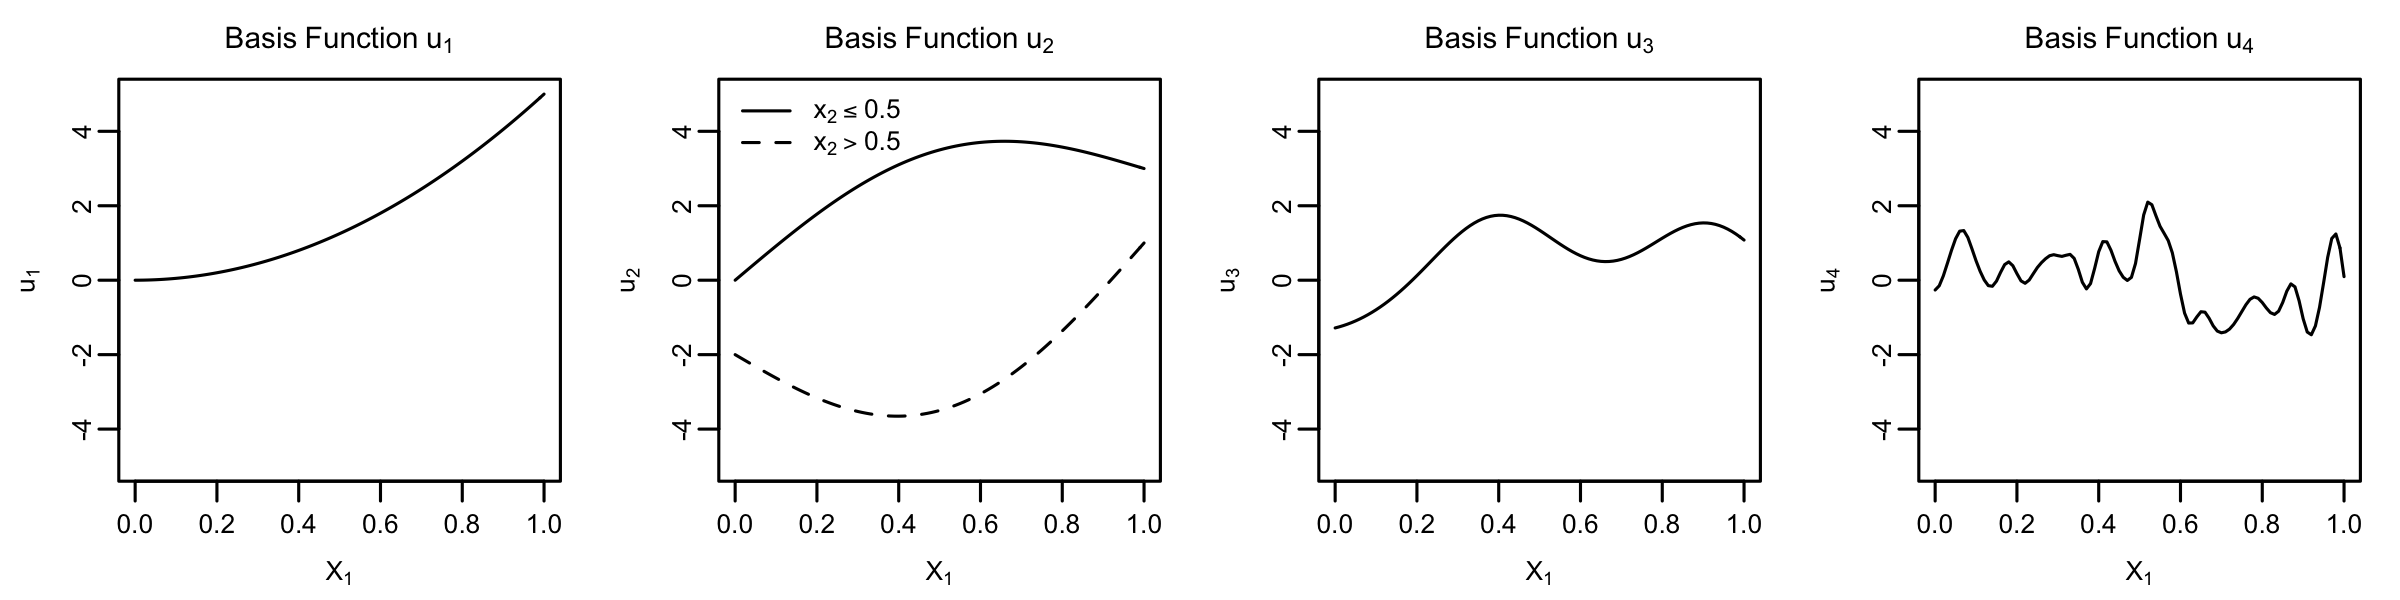
\includegraphics[width = \textwidth]{../images/toy_example_basis.png}
\caption{Basis functions used to generate toy dataset}
\label{fig:toy_example_basis}
\end{figure}

To construct $f_{1}$ and $f_{2},$ we drew each $\phi_{k,d} \sim N(0,1)$ and then set $y_{i,1} = f_{1}(\bx_{i}) + 0.75\epsilon_{i,1}$ and $y_{i,2} = f_{2}(\bx_{i}) + 0.5\epsilon_{i,2}$ where $\epsilon_{i,1}, \epsilon_{i,2} \sim N(0,1).$
Figure~\ref{fig:toy_example_data} plots $f_{1}$ and $f_{2}$ along with the observed data from both tasks.

\begin{figure}[H]
\centering
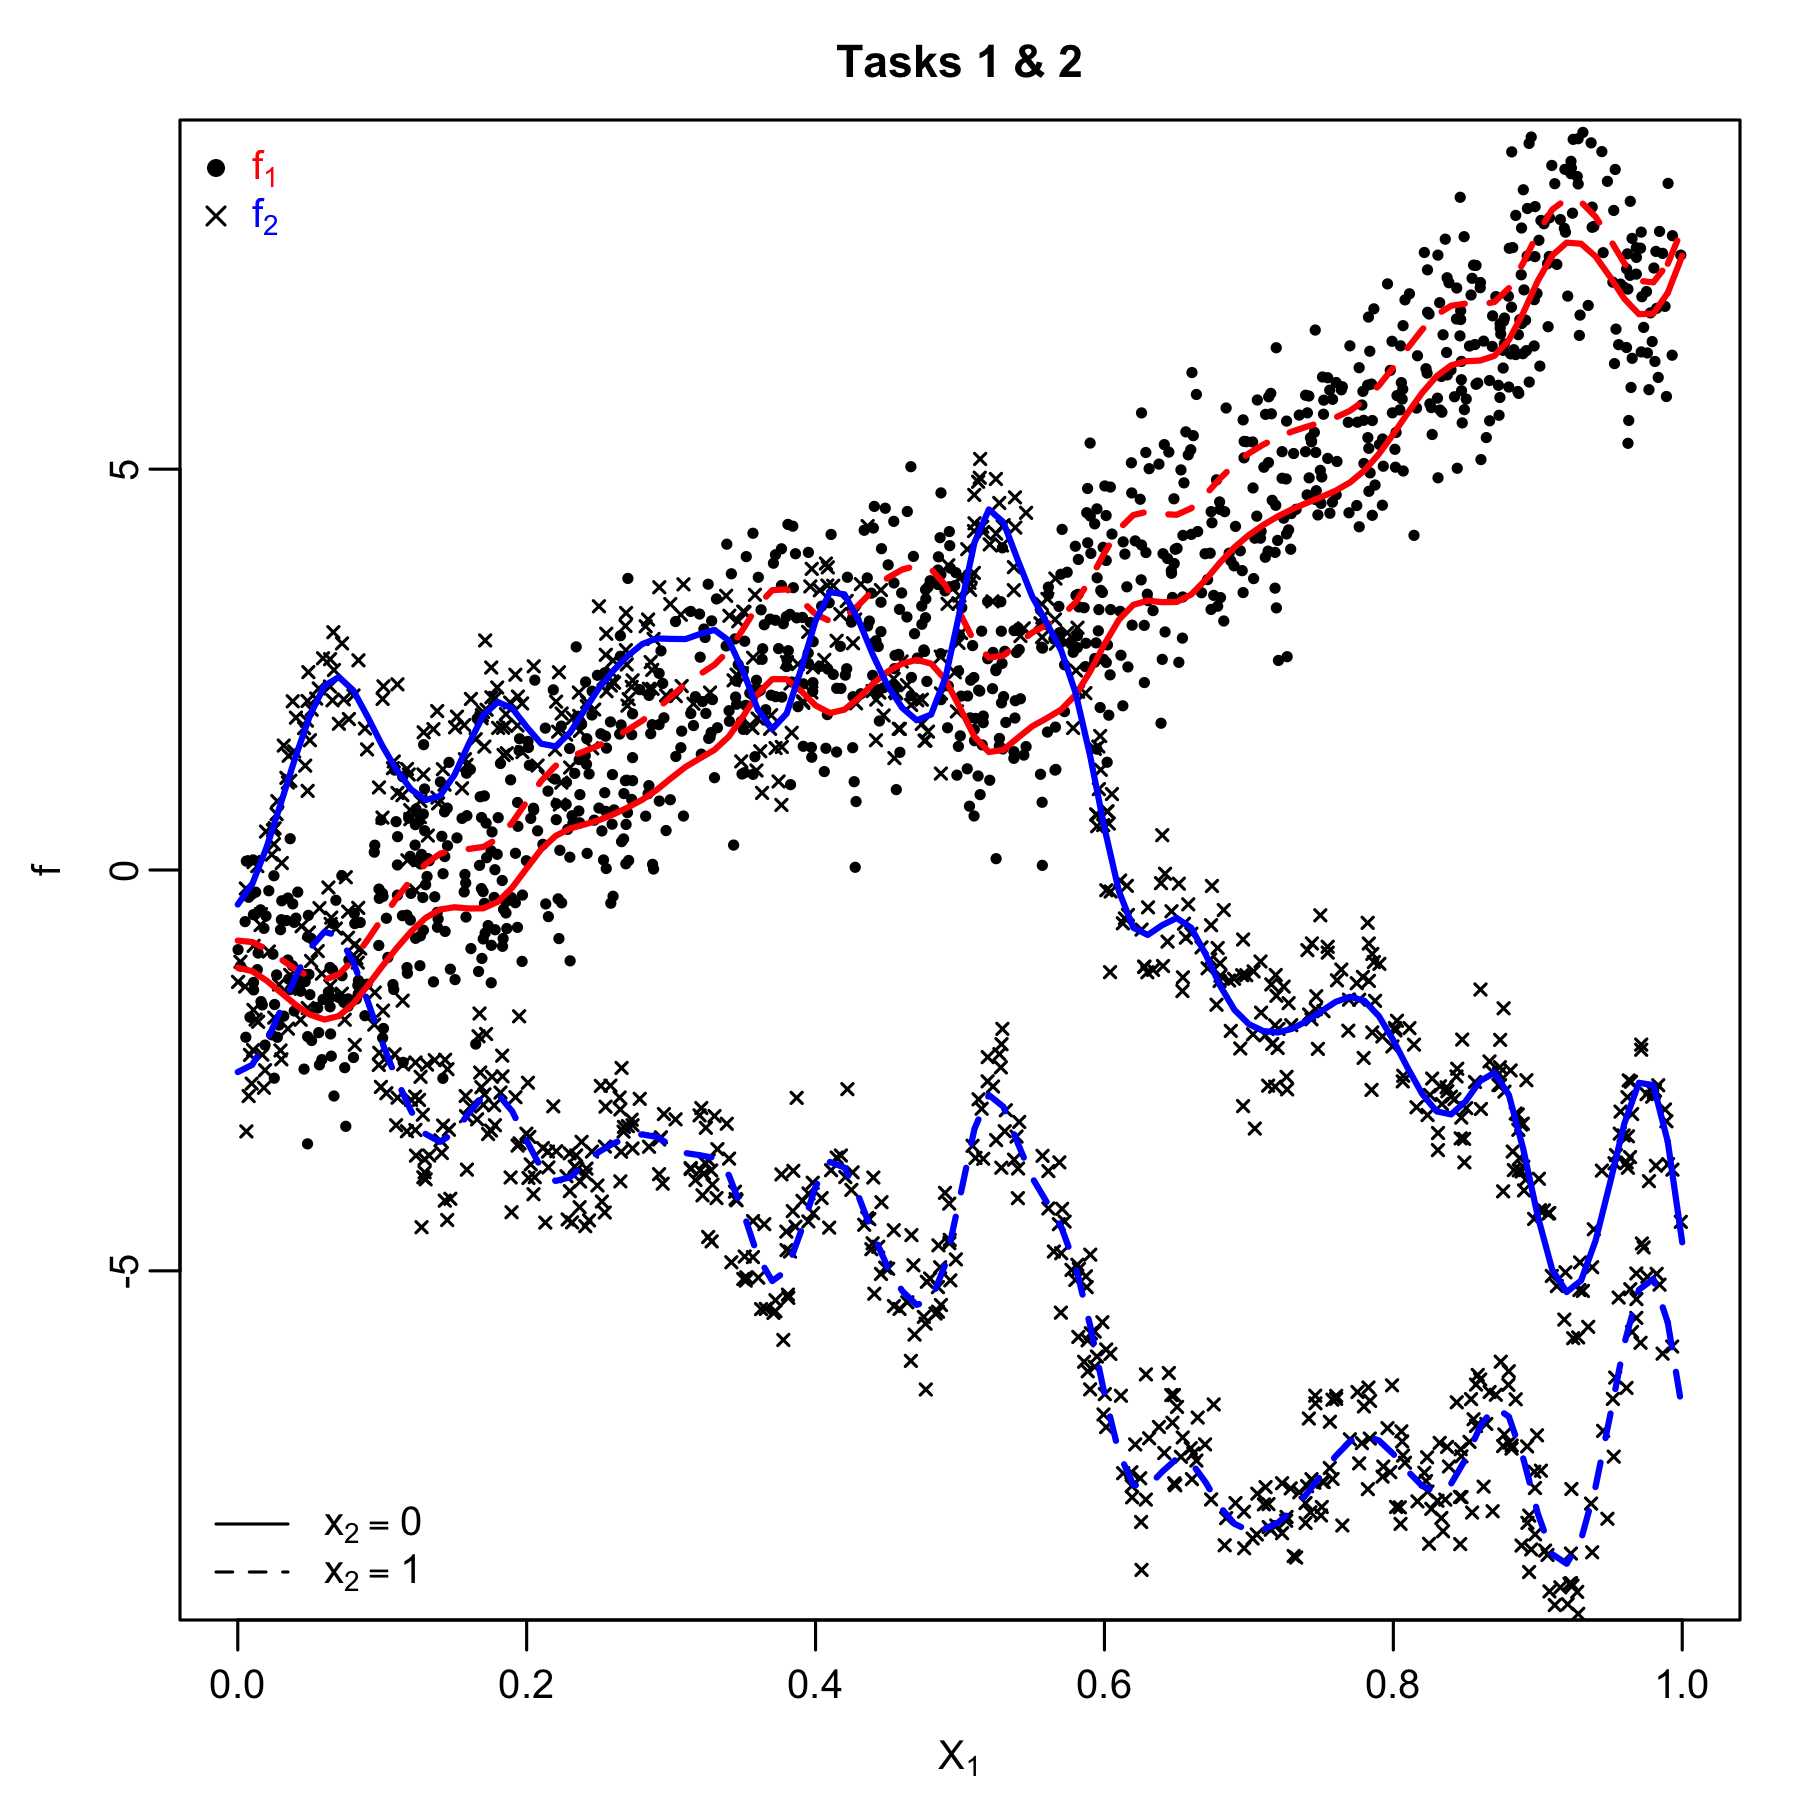
\includegraphics[width = 0.75\textwidth]{../images/toy_example_data.png}
\caption{Two tasks, $f_{1}$ (red) and $f_{2}$ (blue). Realizations from $f_{1}$ are plotted with $\bullet$'s while realizations from $f_{2}$ are plotted with $\times$'s.}
\label{fig:toy_example_data}
\end{figure}

Recall that the main idea is to leverage the fact that $f_{1}$ and $f_{2}$ are dependent while learning them.
As a baseline, we see how well we can learn these two functions separately, using individual BART fits.
Figure~\ref{fig:toy_example_sepBART_fits} shows the posterior mean $f_{1}$ and $f_{2}$ using the default hyper-parameter specifications.

\begin{figure}[H]
\centering
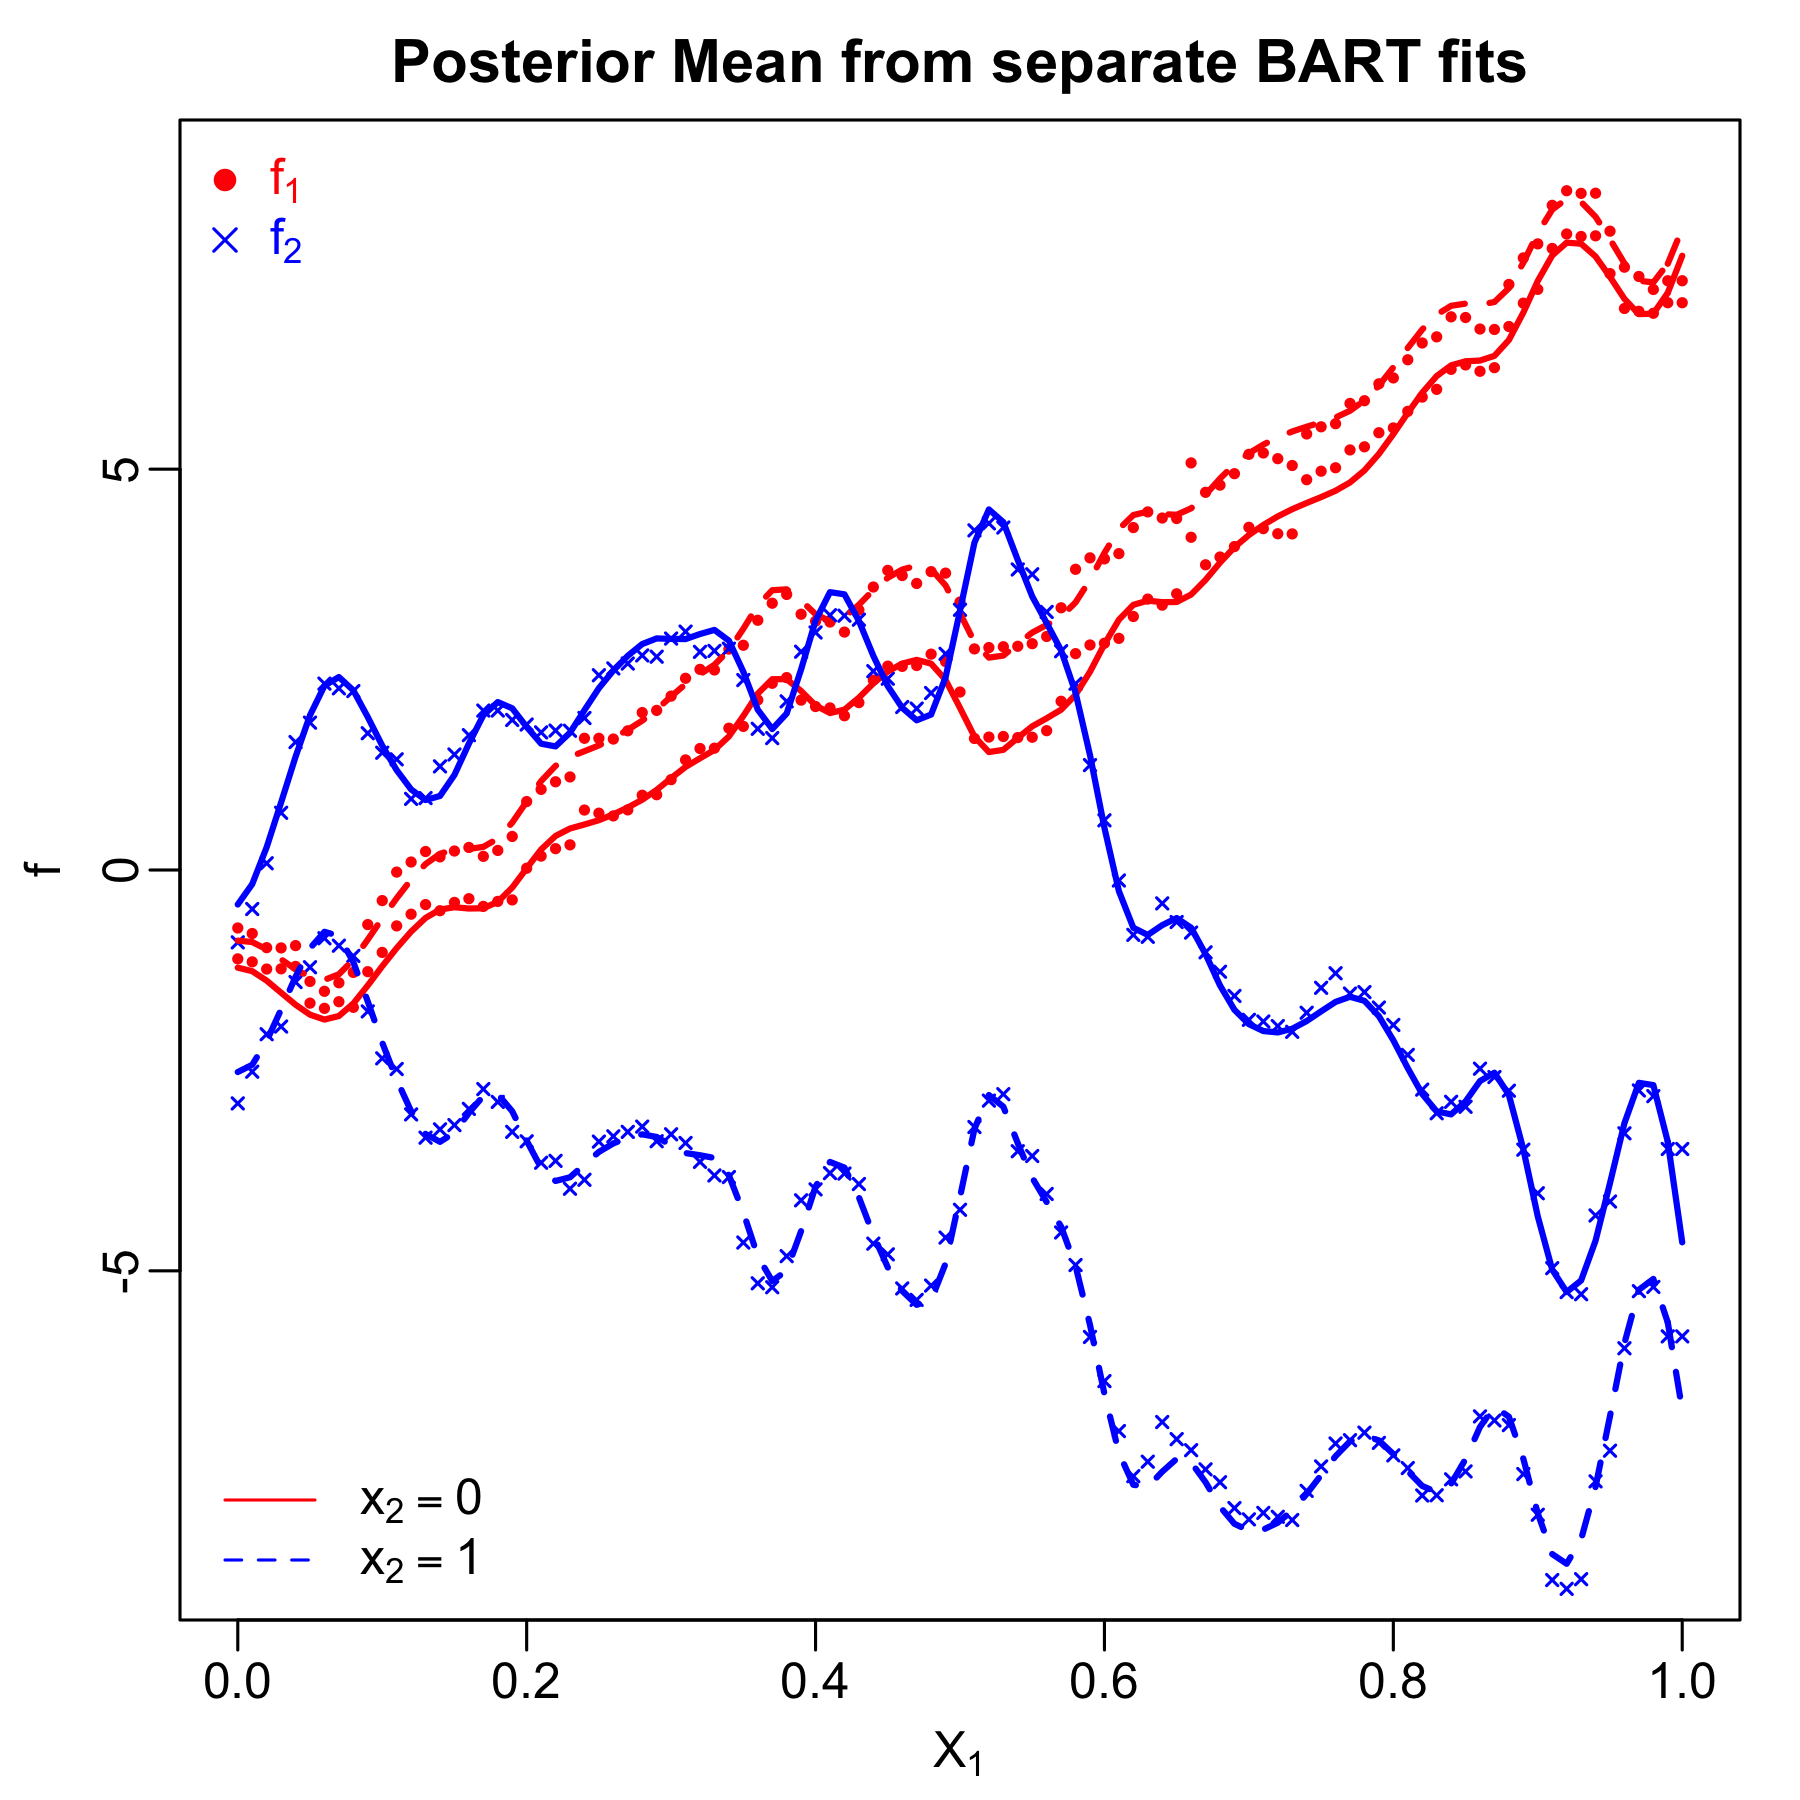
\includegraphics[width = 0.75\textwidth]{../images/toy_example_sepBART_fits.png}
\caption{Points are the posterior means of $f_{1}$ and $f_{2}$ resulting from separate BART fits with default hyper-parameters. The true functions are plotted as lines.}
\label{fig:toy_example_sepBART_fits}
\end{figure}

The in-sample root mean-squared errors $\left(n^{-1}\sum{\left(\hat{f}(\bx_{i}) - f(\bx_{i})\right)^{2}}\right)^{1/2}$ are 0.169 for task 1 and 0.168 for task 2.
The out-of-sample RMSEs are 0.181 and 0.202, respectively.
The hope is that our proposed models can achieve better performance than these baselines.



%\subsection{Missing observations}
%Above, we formulated our procedure with an eye towards missing data.
%In this experiment we consider varying the amount of missing data from each task.

%We can also consider a slightly more complicated two-dimensional example.
%We begin with 
%\begin{align*}
%u_{1}(x_{1},x_{2}) &= 3(x_{1} - x_{2})^{2} \times \max\left\{x_{1},x_{2}\right\} \\
%u_{2}(x_{1},x_{2}) &= 3x_{1} + (2 - 3
%\end{align*}


\newpage

\begin{comment}
\section{Multi-task GPs}
\label{sec:multi_task_gps}

There are two main approaches to multi-task learning with GP, those based on a super-position of independent latent basis functions and those based on process convolutions \citep{Alvarez2012}.
Here, we review the first approach and note several equivalent representations used in the machine learning literature.
We note that these representations are well-known and are comprehensively summarized in Section 4 of \citet{Alvarez2012}, which also reviews process convolutions. 

We start with the semiparametric latent factor model (SFLM) of \citet{Teh2005}, which introduces $D$ independent functions $u_{1}, \ldots, u_{D},$ with $u_{d} \sim \text{GP}(0, k_{d})$ and vectors $\phi_{1}, \ldots, \phi_{D} \in \R^{q}$ and expresses
$$
f_{k}(\bx) = \sum_{d = 1}^{D}{\phi_{k,d}u_{d}(\bx)}
$$
More concisely, we write $\bf = \Phi \bu,$ where $\Phi = (\phi_{k,d}) \in \R^{q \times d}$ and $\phi_{k,d}$ captures the dependence of the $\text{k}^{\text{th}}$ task on the $\text{d}^{\text{th}}$ basis element.

Immediately, we see that for any $\bx$, the vector $\bu(\bx) = (u_{1}(\bx), \ldots, u_{D}(\bx))'$ has a Gaussian distribution with mean zero and covariance matrix $\text{diag}(k_{d}(\bx,\bx)).$
This in turn immediately implies that the realizations of the $q$ tasks at $\bx,$ $\bf(\bx) = (f_{1}(\bx), \ldots, f_{q}(\bx))$ is jointly Gaussian with covariance matrix $\Phi\text{diag}(k_{d}(\bx,\bx))\Phi^{\top}.$
The fact that the $u_{d}$'s are realizations from independent Gaussian processes allows us to say much more.
In particular, for any collection of inputs $\bx_{1}, \ldots, \bx_{n},$  let $K_{d}$ be $n \times n$ matrices with entries $k_{d}(\bx_{i}, \bx_{j}).$
Further, let $\bu_{n}$ be the $nD\times1$ vector concatenating the elements of $\bu(\bx_{1}), \ldots, \bu(\bx_{n}):$
$$
\bu_{n} = (u_{1}(\bx_{1}), \ldots, u_{1}(\bx_{n}), \ldots, u_{D}(\bx_{1}), \ldots, u_{D}(\bx_{n}))^{\top}
$$. 
We have $\bu_{n} \sim N(0,\Sigma_{u})$ where is an $nD \times nD$ block-diagonal matrix with diagonal blocks $K_{1}, \ldots, K_{D}.$
Now if we similarly concatenate $\bf(\bx_{1}), \ldots, \bf(\bx_{n})$ into the $nq \times 1$ vector $\bf_{n},$ we have $\bf_{n} = (\Phi \otimes I_{n})\bu_{n},$ implying that $\bf_{n}$ follows a multivariate Gaussian distribution.
\textcolor{blue}{[skd]: if we think about it for a moment, this is actually a pretty strong distributional assumption. In the context of physiological time series, not only are we assuming that the realizations from each series at a given time point are jointly Gaussians, we are also assuming that realizations across time points are jointly Gaussian. It's important to stress that this is a consequence of the GP prior on the $u_{d}$'s and it may not have any fidelity to the data.}

The representation $\bf = \Phi \bu$ allows us to quickly compute the cross-covariance
\begin{align*}
\text{Cov}(f_{k}(\bx), f_{k'}(\bx')) &= \text{Cov}\left(\sum_{d = 1}^{D}{\phi_{k,d}u_{d}(\bx)},\sum_{d' = 1}^{D}{\phi_{k',d'}u_{d'}(\bx')}\right) \\
&= \sum_{d,d'}{\phi_{k,d}\phi_{k',d'}\text{Cov}(u_{d}(\bx), u_{d'}(\bx'))} \\
&= \sum_{d = 1}^{D}{\phi_{k,d}\phi_{k',d}k_{d}(\bx,\bx')},
\end{align*}
where in the first line we are using the fact that the $u_{d}$'s are independent and in the second line we are using the fact that $\text{Cov}(u_{d}(\bx), u_{d'}(\bx)) = k_{d}(\bx,\bx').$
\citet{Teh2005} take an empirical Bayes approach to estimating $\Phi$ within in a larger variational approximation scheme to estimate $\bf.$
In contrast, \citet{Titsias2011} place spike-and-slab priors on the elements of $\Phi,$ $\phi_{d,k} \sim (1 - \pi)\delta_{0}(\phi_{d,k}) + \pi\text{N}(0, \sigma^{2}_{\phi}),$ and propose a variational approximation to the posterior of $(\Phi, \pi, \bu_{n}).$
They further describe a Gibbs sampler for directly sampling from the posterior.

If we take $q = D$ and further suppose that the $u_{d}$'s are in fact i.i.d., then the SFLM becomes the intrinsic correlation model (ICM) studied by \citet{Bonilla2008} that originates in the geostatistics literature (\textcolor{blue}{[skd]: there are a few textbook references given for these but I haven't yet tracked them down}).
In this case, the cross-correlation term has a simple, separable form
$$
\text{Cov}(f_{k}(\bx), f_{k'}(\bx')) = b_{k,k'}k(\bx,\bx')
$$
with $B = \Phi\Phi^{\top}.$
\citet{Bonilla2008} treats the matrix $B$ as a hyperparameter and estimates it, along with the basis kernel hyperparameters, in an empirical Bayes fashion.
Somewhat more recently, \citet{Swersky2013} use a slice sampler within a larger MCMC simulation to draw approximate samples of $B$ from its posterior distribution.

A further elaboration of the SFLM and ICM is the linear model of coregionalization (LCM), which also has its roots in the geostatistics literature.
Specifically, suppose that instead of introducing a single $u_{d} \sim \text{GP}(0,k_{d})$ in the SFLM, we actually introduce $R_{d}$ independent realizations $u^{(1)}_{d}, \ldots, u^{(r_{d})}_{d}$ and express
$$
f_{k}(\bx) = \sum_{d = 1}^{D}{\sum_{r = 1}^{R_{d}}{\phi^{(r)}_{d,k}u_{d}(\bx)}}
$$

For each $d = 1, \ldots, D,$ we may define $B_{d} = \sum_{r = 1}^{R_{d}}{\phi^(r)_{d}\phi^{(r)\top}_{d}}$ so that
$$
\text{Cov}(f_{k}(\bx), f_{k'}(\bx')) = \sum_{d = 1}^{D}{b_{d,k,k'}k_{d}(\bx,\bx')}
$$
\end{comment}
%\subsection{Examples}
%Here we visualize realizations from these models, largely following the example of \citet{Alvarez2012}.
\begin{comment}
\section{Review of Bayesian Additive Regression Trees}
\label{sec:bart_review}

\textcolor{blue}{[skd]: if this were a paper, now would be a good time to list limitations of GPs in general. Probably the most salient are: (i) even with fully specified kernels, training GPs exactly is computationally prohibitive and it's not obvious how close any of the approximations come to the exact posterior, (ii) specifying kernels is difficult. And in the case of the LMC, one has to specify D of them. With relatively vague ideas about how the tasks evolve, this seems like a really hard problem. The last limitation is that inference is likely sensitive to kernel hyperparameters, and learning them with Empirical Bayes is no longer coherently Bayes. This may not matter to many people though.}

As an alternative to GPs, we consider the Bayesian Additive Regression Trees (BART) approach of \citet{Chipman2010}.
In the single task model, with $y_{i} = f(\bx_{i}) + \sigma\epsilon_{i}, \epsilon_{i} \sim N(0,1),$ BART approximates $f$ as sum of $m$ regression trees.
To set our notation, let $T$ denote a binary decision tree partitioning $\R^{p}$ that consists of a collection of interior nodes and $L(T)$ terminal or \textit{leaf} nodes.
To each interior node of $T$ we associate an axis-aligned decision rule of the form $\left\{x_{j} < c \right\}$ or $\left\{x_{j} \geq c \right\}.$
Note that $T$ defines a partition of $\R^{p}$ into $L(T)$ cells.
Let $\ell(\bx,T)$ be the function that returns the index of the partition cell containing $\bx.$
To form a regression tree from $T,$ we associate a parameter $\mu_{\ell}$ to each leaf of $T.$
Given $T,$ denote $M = \left\{\mu_{1}, \ldots, \mu_{L(T)}\right\}.$
We will refer to the pair $\left(T, M \right)$ as a regression tree and define the evaluation function
$$
g(\bx; T,M) = \mu_{\ell(\bx,T)},
$$
which maps $\bx$ to the leaf parameter corresponding to the partition cell $\ell(\bx,T).$
\textcolor{blue}{[skd]: this is exceptionally verbose. A picture is way more intuitive.}

At the heart of BART is the approximation
$$
f(\bx) \approx \sum_{t = 1}^{m}{g(\bx; T_{(t)}, M_{(t)})}.
$$
and a prior on the collection $(\T,\M) = \left\{(T_{1}, M_{1}), \ldots, (T_{m}, M_{m})\right\}$ which implicitly defines a prior over the function $f.$
The regression trees $(T_{t},M_{t})$ are modeled \textit{a priori} independent. 
The prior on regression trees $(T,M)$ consists of two parts, a prior on the leaf parameters $M$ conditional on $T$ and a prior on the decision tree $T.$
Conditional on $T,$ \citet{Chipman2010} models $\mu_{\ell} \sim N(\mu_{\mu},\sigma^{2}_{\mu})$ independently for $\ell = 1, \ldots, L(T).$
They further propose a branching process prior for $T$ consisting of three parts: the probability that a node at depth $d$ is non-terminal and a distribution for the decision rule at each interior node.
They specifically set the probability that a node at depth $d$ is non-terminal to be $\alpha(1 + d)^{-\beta}$ and pick the splitting rule uniformly from the set of all available splitting rules.
Together, these parts induce a prior over the space of all functions which serves to regularize $f.$
We will write $f \sim \text{BART}(m, \alpha, \beta, \mu_{\mu}, \sigma_{\mu}).$
\end{comment}


\begin{comment}
The success of BART derives largely from the effect ``default'' hyperparameter settings suggested by \citet{Chipman2010} that give ``reasonable baseline levels of performance without requiring tuning by the user.''
Specifically \citet{Chipman2010} recommend setting $\alpha = 0.95$ and $\beta = 2$ so that with the decision tree $T$ has depth four or less with high prior probability.
Note that the induced prior on $f(\bx)$ is $N(m\mu_{\mu}, \sigma^{2}_{\mu})$ and they recommend setting $\mu_{\mu}$ and $\sigma_{\mu}$ so that this normal distribution assigns substantial prior probability to the range of the data.
To this end, assuming the data is standardized to have mean 0 and variance 1, we can set $\mu_{\mu} = 0$ and parametrize $\sigma_{\mu} = \kappa^{-1}\text{range}(\by).$
\citet{Chipman2010} recommend setting $\kappa = 2$ by default.


To approximate draws from the posterior of $f$, we first simulate draws from the posterior over the regression trees $(T_{t}, M_{t})$ with a Gibbs sampler.
See \citet{Chipman2010}, \citet{Pratola2016}, and \citet{Linero2017} for further details.
\end{comment}

%\subsection{Example}
% Can we visualizes draws from BART
% Maybe use examples from our uniBART method here.

%Admittedly these examples are simple but they do highlight the effectiveness of BART
\begin{comment}
\subsection{Connection between BART and Kernel Methods}

This section is mostly drawn from Section 5.2 of \citet{Linero2017}.
Suppose that $u \sim \text{BART}(m,\alpha, \beta, 0, \sigma_{\mu}).$
We observe immediately that the implied prior on $u(\bx)$ is $N(0, m\sigma^{2}_{\mu}).$
Further, we compute
\begin{align*}
\text{Cov}(u(\bx), u(\bx')) &= \sum_{t,t'}{\text{Cov}(g(\bx; T_{t},M_{t}), g(\bx', T_{t'},M_{t'}))} \\
&= m\text{Cov}(\mu_{\ell(\bx,T)},\mu_{\ell(\bx',T)}) \\
& = m\sigma^{2}_{\mu}\P(\bx \sim \bx')
\end{align*}
where $\bx \sim \bx'$ if $\bx$ and $\bx'$ are assigned to the same leaf in the decision tree $T$ (i.e. $\ell(\bx,T) = \ell(\bx',T)$).
In this calculation, we are first using the fact the trees are independent and then using the fact that $\mu_{\ell}$'s corresponding to different leaves of $T$ are independent.

\citet{Linero2017} considers a slight reparametrization of the BART prior and appeals to the multivariate central limit theorem to show that as the number of trees $m$ increases, the vector $(u(\bx_{1}), \ldots, u(\bx_{n}))$ converges weakly to a multivariate normal with covariance matrix with entries proportional to $\P(\bx \sim \bx').$
He goes on to state a heuristic theorem that as $m \rightarrow \infty,$ $u$ converges weakly to a realization from a Gaussian process with kernel function proportional to $\P(\bx \sim \bx').$
\textcolor{blue}{[skd]: I'm inclined to believe this but I'm not 100\% convinced that $\P(\bx \sim \bx')$ is a positive definite kernel. If it is, then it's cool to note that BART is an approximation to a very specific GP.}

At this point, it is worth drawing an important distinction between BART and GPs.
Under both formulations, $\bf(\bx)$ follows a multivariate Gaussian distribution.
However, under the GP formulation for any other $\bx',$ the distribution of $(\bf(\bx), \bf(\bx'))$ is also Gaussian.
With BART, the joint distribution of $(\bf(\bx), \bf(\bx'))$ converges to a multivariate Gaussian as the number of trees increases $m \rightarrow \infty$ but for any finite $m$ it is not Gaussian. 
\end{comment}


\begin{comment} 
 
\newpage
\subsection{Some existing formulations}
\label{sec:existing_work}


\textcolor{blue}{[skd]: The punchline is that many of the models are are based on a super-position of latent Gaussian processes. After writing this up I found this more or less already expressed at this Wikipedia page: \url{https://en.wikipedia.org/wiki/Kernel_methods_for_vector_output\#Linear_model_of_coregionalization_(LMC)}}

We start with the semiparametric latent factor model (SLFM) of \citet{Teh2005}, which introduces $D$ independent functions $u_{1}, \ldots, u_{D}$ where $u_{d} \sim \text{GP}(0, k_{d})$ and models independently for each $i = 1, \ldots, n$,
$$
\bf(\bx_{i}) = \Phi\bu(\bx_{i})
$$
where $\Phi = (\phi_{k,d}) \in \R^{q \times D}$ is a fixed matrix.
In this formulation, we compute
\begin{align*}
\text{Cov}(f_{k}(\bx), f_{k'}(\bx')) &= \text{Cov}\left(\sum_{d = 1}^{D}{\phi_{kd}u_{d}(\bx)},\sum_{d' = 1}^{D}{\phi_{k'd'}u_{d'}(\bx')}\right) \\
&= \sum_{d,d'}{\phi_{kd}\phi_{k'd'}\text{Cov}(u_{d}(\bx), u_{d'}(\bx'))} \\
&= \sum_{d = 1}^{D}{\phi_{kd}\phi_{k'd}k_{d}(\bx,\bx')},
\end{align*}
where the last equality follows from the independence of the latent functions $u_{d}.$

Another formulation is the intrinsic correlation model which writes
$$
\text{Cov}(f_{k}(\bx), f_{k'}(\bx')) = B_{k,k'}k(\bx,\bx'),
$$
where $B$ is a symmetric positive semi-definite matrix that captures the relationships between tasks and $k$ is a kernel function capturing the similarities of the inputs.
We recognize this as a special case of the SLFM: to wit, say we decompose
$$
B = \sum_{d = 1}^{D}{\beta_{d}\beta_{d}^{\top}}
$$
so that $b_{ij} = \sum_{d}{\beta_{di}\beta_{dj}}$ where each $\beta_{d} \in \R^{q}.$

Consider introducing $u_{1}, \ldots, u_{q}$ which are independent draws from $\text{GP}(0,k)$ and model
\begin{equation}
\label{eq:imc_representation}
f_{k} = \sum_{d = 1}^{D}{\beta_{d,k}u_{d}}.
\end{equation}
We compute
$$
\text{Cov}(f_{k}(\bx), f_{k'}(\bx)) = \sum_{d = 1}^{D}{\beta_{d,k}\beta_{d,k'}k(\bx,\bx')} = b_{k,k'}k(\bx,\bx').
$$
%Put another way, the intrinsic model of correlation is essentially representing each $f_{k}$ as a linear combination of latent basis functions which are \textit{a priori} iid from the same GP.
% We need to be extra sure this is the case.
% In particular, what is the joint distribution


This ICM model was studied by \citet{Bonilla2008}, who also notes this connection to the SLFM.
If we require that $B$ was positive definite, then we would have $D = q.$
In other words, the ICM corresponds to introducing a latent basis of $q$ draws from a $\text{GP}(0,k)$ and expressing each $f_{k}$ as a linear combination of these basis elements.
In \citet{Bonilla2008}, $B$ is treated as a hyperparameter and is set by maximizing the marginal likelihood.
%\textcolor{blue}{[skd]: I've also seen some people say that all of the off-diagonal elements of $B$ are positive, which seems arbitrarily restrictive but that's a different matter...}
Somewhat more recently, \citet{Swersky2013} deployed a slice sampler to estimate $B.$

\citet{Bonilla2008} also mentions in passing the linear coregionalization model (LCM), which is a sum of ICM models.
\citet{Cheng2018} use an LCM to model physiological time-series data. 
In the LCM, we specify matrices $B^{(1)}, \ldots, B^{(C)}$ and corresponding kernel functions $k_{1}, \ldots, k_{C}$ and model 
$$
\text{Cov}(f_{k}(\bx), f_{k'}(\bx')) = \sum_{c = 1}^{C}{B^{(c)}_{k,k'}k_{c}(\bx,\bx')},
$$
Assuming that each $B^{(c)}$ is positive definite, we can get representation quite similar to that in Equation~\eqref{eq:imc_representation}
$$
f_{k}(\bx) = \sum_{c = 1}^{C}{\sum_{d = 1}^{q}{\beta^{(c)}_{d,k}u^{(c)}_{d}(\bx)}}
$$
where $B^{(c)} = \sum_{d = 1}^{q}{\beta^{(c)}_{d}\beta^{(c)\top}_{d}},$ and for each $c = 1, \ldots, C,$ the functions $u_{d}^{(c)}$ are iid realizations of a $\text{GP}(0, k_{c}).$

Some passing remarks:
\begin{itemize}

\item{\citet{Futoma2017} also consider an LMC, stating `` we find $C = 3$ works well in practice'' but don't provide any guidance about selecting the covariance kernel functions $k_{c}$}
\item{\citet{Cheng2018} use a spectral mixture kernel which they parametrize as
$$
\kappa_{q}(x,x') = \exp\left\{-2v_{q}\pi^{2}\lVert x - x' \rVert^{2}_{2}\right\}\cos\left(2\pi\lVert x - x; \rVert_{2}\mu_{q}\right)
$$
}

\end{itemize}
\end{comment}
\begin{comment}
\section{LMC BART}

Each of the frameworks above expresses the function $f_{k}$ as linear combinations of a set of independent basis functions, which are given Gaussian process priors.
We now consider a variant in which we replace the GP priors with BART priors.

% Start with the analog of the SLFM -- let the u_{d}'s be regression trees -- equivalent to $BART(m, alpha, beta, \sigma^{2}_{\mu}, \mu_{\mu})$
% wlog \mu_{\mu} = 0 and \sigma^{2}_{\mu} is what we would expect it to be
% 

% Written like this, I think we recover something similar to what Linero 2018 does.
% I believe *marginally* his model is equivalent to having a sum of regression trees with a vector of $\Sigma_{\mu}$ at the base
% If we go with that, and take the decomposition of $\Sigma_{\mu}$ we will recover a SLFM-RT model

% Extending a bit, we could consider a SLFM with BART functions instead of regression trees
% We may also try deeper trees (i.e. varying the BART priors) but this seems a bit more aggressive


\subsection{Review of BART}

We briefly review the main ideas of BART.
Suppose that we observe data $(\bx_{1},y_{1}), \ldots, (\bx_{n}, y_{n})$ with $y_{i} = f(\bx_{i}) + \epsilon_{i}, \epsilon_{i} \sim N(0,\sigma^{2})$ and wish to estimate the unknown function $f.$
The main idea of BART is to approximate $f$ as the sum of $m$ regression trees.
To set our notation, let $T$ denote a binary decision tree partitioning $\R^{p}$ that consists of a collection of interior nodes and $L(T)$ terminal or \textit{leaf} nodes.
Each decision rule corresponding to the interior nodes of $T$ are binary splits of the form $\left\{x_{i} < c\right\}$ or $\left\{x_{i} \geq c \right\}.$
Further let $M = \left\{\mu_{1}, \ldots, \mu_{L(T)}\right\}$ be a set of parameters associate with each of the terminal nodes of $T.$
Let $\ell(\bx; T)$ be the function that returns the index of the terminal node of $T$ to which $\bx$ belongs and let $I(\ell,T)$ be the collection of indices $i$ for which $\ell(\bx_{i},T) = \ell.$
Abusing our nomenclature slightly, we will refer to the pair $\left(T, M\right)$ as a tree and the single $T$ as a decision tree.
With this notation, we define the function
$$
g(\bx; T,M) = \mu_{\ell(\bx, T)}
$$
to be the evaluation of the regression tree $(T,M)$ at $\bx.$

At the heart of BART is the approximation
$$
f(\bx) \approx \sum_{t = 1}^{m}{g(\bx; T^{(t)}, M^{(t)})}.
$$
and a prior on the collection $(\T,\M) = \left\{(T_{1}, M_{1}), \ldots, (T_{m}, M_{m})\right\}$ which implicitly defines a prior over the function $f.$
\citet{Chipman2010} propose
\begin{align*}
\pi(\T, \M) &= \prod_{t = 1}^{m}{\pi(M_{t}|T_{t})\pi(T_{t})} \\
\pi(M_{t} | T_{t}) &= \prod_{\ell = 1}^{L(T_{t})}{\pi(\mu_{\ell,t}|T_{t})}
\end{align*}
In other words, conditional on the regression tree, the terminal node parameters are independent.
Moreover, each $\mu_{\ell,t}$ is given a $N(0,\sigma^{2}_{\mu})$ prior with $\sigma^{2}_{\mu}$ specified (see below).
The induced prior on $f(\bx) \in N(0, m\sigma^{2}_{\mu})$ and \citet{Chipman2010} suggest setting
$$
\sigma = \frac{\text{range}(y)}{k\sqrt{m}}
$$
so that \textit{a priori}, the range of the data $y$ is covered by $k$ standard deviations. 
The prior on $T$ is set in a way to discourage individual decision trees from being too deep and potentially over-fitting the data.

If $u$ is a draw from a BART prior, we compute
$$
\text{Cov}(u(\bx), u(\bx')) = \sum_{t,t'}{\text{Cov}(g(x,T_{t},M_{t}), g(x', T_{t'}, M_{t'}))} = \sum_{t = 1}^{m}{\text{Cov}(\mu_{\ell(x,T_{t})}, \mu_{\ell(x,T_{t'})})} ,
$$
where we are using the fact that the regression trees $(T_{t}, M_{t})$ are independent.
Now if $\ell(x,T_{t}) = \ell(x,T_{t'})$ the covariance above is just $\sigma^{2}_{\mu}$ and if $\ell(x,T_{t}) \neq \ell(x,T_{t'}),$ the covariance is 0 since the terminal node parameters are \textit{a priori} independent.
We therefore have
$$
\text{Cov}(u(\bx), u(\bx')) = m\sigma^{2}_{\mu}\P(\bx \sim \bx')
$$
where we write $\bx \sim \bx'$ iff $\ell(\bx,T) = \ell(\bx',T)$ and the probability is taken over the process generating the regression trees $T.$
This highlights an interesting connection between BART and kernel methods that is described in some more detail in \citet{Linero2017}.
If we let $\tilde{\sigma}^{2}_{\mu} = m\sigma^{2}_{\mu},$ we see
$$
u(\bx) = \sqrt{m} \times \left(m^{-1}\sum_{t = 1}^{m}{g(\bx; T_{t}, M_{t})}\right).
$$
So by the multivariate CLT, as $m\rightarrow \infty,$ we conclude
$$
(u(\bx_{1}), \ldots, u(\bx_{n}))^{\top} \rightarrow N(0, \Sigma)
$$
where $\Sigma_{ij} = \tilde{\sigma}^{2}_{\mu}\P(\bx_{i} \sim \bx_{j}).$
\citet{Linero2017} goes further to state a heuristic theorem that for a collection of inputs $\mathcal{X},$ the collection $\left\{u(\bx): \bx \in \mathcal{X}\right\}$ converges to a GP with mean 0 and covariance kernel $k(\bx,\bx') = \tilde{\sigma}^{2}_{\mu}\P(\bx \sim \bx').$
\textcolor{blue}{[skd]: I'm inclined to believe this but I'm not yet 100\% convinced that the kerne$\P(\bx \sim \bx')$ is a positive definite kernel. If it is, we can view BART as an approximation to a specific GP}

\subsection{BART model for multi-output data}
\label{sec:multioutput_bart}

% Maybe start by presenting the fully saturated model. If we don't link them together, it's equivalent to training separate models
% Another thing we can do

% We take a slightly different approach.
% In our model, we don't have a joint gaussian distribution for (f_1(x), f_2(x), ..., f_q(x))
% I believe Linero's model is equivalent to saying that the vector f can be expressed as sum of regression trees with \textit{vector}-valued terminal node parameters


Following the general form of the IMC, we introduce latent functions $u_{1}, \ldots, u_{D}$ iid from a BART prior and vectors $\phi_{1}, \ldots, \phi_{q} \in \R^{d}$ and approximate
\begin{equation}
\label{eq:imc_bart}
f_{k}(\bx) = \sum_{d = 1}^{D}{\phi_{k,d}u_{d}(\bx)} = \sum_{d = 1}^{D}{\phi_{k,d}\sum_{t = 1}^{m}{g(\bx, T_{t}^{(d)}, M_{t}^{(d)})}}
\end{equation}
With this representation, we have for each $k = 1, \ldots, K,$
$$
f_{k}(\bx) \sim N(0, \lVert \phi_{k}\rVert_{2}^{2}\sigma^{2}_{\mu}).
$$

If we let $\Phi \in \R^{q \times D}$ be the matrix whose $\text{k}^{\text{th}}$ row is $\phi_{k},$ we can more concisely write our model as
$$
\bf(\bx) = \Phi\bu \sim N(0, \sigma^{2}_{\mu}\Phi\Phi^{\top})
$$

% Is this actually equivalent to what we are doing?
% I'm not convinced of anything anymore!

% Specifically: is the joint distribution of f(bx) Gaussian in my case?
% If I write it as a linear combination of Gaussians then I totally buy it.
% But if I instead had f_1 = 1 * u_1, f_2 = 2 * u_1 then (f_1, f_2) = [1 ;0 // 2; 0] * (u_1, u_2) which I guess still technically have a gaussian distirubtion, it's just degenerate


% In which case I think the punch line is that if we take an LMC where the latent basis functions are regression trees, we recover exactly Linero's model, with a suitable choice of beta.
% Putting a prior on beta is somewhat nice because it now let's us ``learn'' the correlations between tasks.
% Fixing the Sigma is not necessarily helpful
Using the fact that the latent functions $u_{d}$ are independent, we can compute the conditional cross-covariance given $\Phi$
$$
\text{Cov}(f_{k}(\bx),f_{k'}(\bx') \mid \Phi) = m\sigma^{2}_{\mu}\P(\bx\sim\bx) \times \sum_{d = 1}^{D}{\phi_{k,d}\phi_{k',d}}
$$

At this point, it bears mentioning that \citet{Linero2018} also considers fitting multiple outputs with a shared ensemble of regression trees.
\end{comment}


\begin{comment}
Conditional on $B = \left[\beta_{1}, \ldots, \beta_{q}\right] \in \R^{d \times q},$ we have
$$
f_{k}(\bx) \sim N(0, \sigma^{2}_{\mu}\lVert \beta_{k}\rVert_{2}^{2}).
$$

Using the fact that the $u_{d}$'s are independent, we can easily compute a conditional cross-covariance
$$
\text{Cov}(f_{k}(\bx), f_{k'}(\bx') \mid B) = \sigma^{2}_{\mu}\P(\bx\sim\bx')\sum_{d = 1}^{D}{\beta_{d,k}\beta_{d,k'}} = m\sigma^{2}_{\mu}\P(\bx\sim\bx')B_{k,k'}
$$


Rather than letting the $u_{1}, \ldots, u_{D}$ be independent draws from a BART prior, we could conceive of them being independent draws from individual regression trees


At this point, it bears mentioning that \citet{Linero2018} also considers fitting multiple outputs with a shared ensemble of regression trees.
Specifically, they express each $f_{k}$ as
$$
f_{k}(\bx) = \sum_{t = 1}^{m}{g(\bx; T_{t}, M_{t}^{(k)})},
$$
where the $M^{(k)}_{t}$ are task-specific terminal nodes parameters and the parameters $\mu_{t,\ell}^{(k)}$ are drawn from a multivariate prior, say $N(0, \Sigma_{\mu}).$
Another way to think about their model is associate to each terminal node a \textit{vector} of parameters, one for each task, which are \textit{a priori} drawn from a multivariate prior (e.g. $N(0,\Sigma_{\mu}).$
In this case, 
$$
\mu_{t,\ell}^{(1)}
$$
For Linero 2018 we have
$$
\text{Cov}(f_{k}(\bx), f_{k'}(\bx')) = \P(\bx \sim \bx') \times \sigma_{\mu,k,k'}
$$

At this point it bears mentioning that \citet{Linero2018} also considers fitting multiple outputs with a shared ensemble of regression trees.
While we are proposing to share a fully specific basis of regression trees across tasks, \citet{Linero2018} shares only the decision trees, allowing each task to have its own set of terminal node parameters. 

It bears mentioning that \citet{Linero2018} also considers fitting multiple outputs with a shared ensemble of regression trees.
However, rather than relying on a fully specified shared basis of regression trees, they only share the decision trees across tasks, and let each task have it's own set of terminal node parameters.
%The implication of this model is ``the features which are useful for approximating $f_{k}(\bx)$ are the same features that are useful for approximating $f_{k'}$''


\textcolor{PennBlue}{[skd]: I'm pretty certain the cross-covariance $\text{Cov}(f_{k}(\bx), f_{k'}(\bx'))$ can be written as sum of the terms $\sigma^{2}_{u}\beta_{d,k}\beta_{d,k'}\P(\ell(\bx;T) = \ell(\bx';T))$ where the last probability is the probability that $\bx$ and $\bx'$ land in the same terminal node of a decision tree.
I'm not 100\% certain that this probability is a valid positive definite kernel but if it is, it would be neat to draw a connection to this ``BART kernel'' and the IMC model. I should mention, Linero has drawn a similar connection between BART and GPs before so I'll follow that reference up}
%$$
%\text{Cov}(f_{k}(\bx), f_{k'}(\bx')) = \sum_{d = 1}^{q}{\beta_{d,k}\beta_{d,k'}\P(\ell(\bx,T_{d}) = \ell(\bx',T_{d}))}
%$$,
%where that probability is the probability that $\bx$ and $\bx'$ end up in the same terminal node of $T_{d}$
%Note in this expression, noting about the the 



\section{A Gibbs Sampler}

For plain vanilla BART, there is a really straightforward Gibbs sampler.
For the model in Equation~\eqref{eq:imc_bart}, we can update the trees keeping $B$ fixed and vice versa.
The tree updates, conditional on $B$ are virtually identical to those in \citet{Chipman2010}. 
Updating $B$ given the regression trees has the flavor of high-dimensional regression.
The trick is to select useful priors on the columns of $B.$

%Here, each $f_{k}$ is being represented as a sum of $mq$ regression trees but the dependence on particular collection
%A perhaps more flexible approach would be to consider
%$$
%f_{k}(\bx) = \sum_{t = 1}^{qm}{\beta_{t,qm}g(\bx;T_{t},M_{t})
%$$
%In other words, each $f_{k}$ is a weighted sum of trees. 


% A version of the IMC would say that we should introduce $mq$ regression trees
% Think of the edge case: that all of the outcome dimensions are independent, we'd want a full set of m trees for each outcome
% Ok now that we have this

% A useful connection is that that this could be viewed as a form of IMC:
% The kernel is somewhat hard to compute and it depends on the tree process
% One could readily imagine that we could depart from the Galton-Watson procedure. But it asks ``do x' and x land in the same partition of the space''
% Important to add the citation to Linero. and note that this kernel cannot actually be evaluated.
\end{comment}
\begin{comment}
\textit{Some questions:}
\begin{itemize}
\item{What is the equivalent characterization of the prior cross-covariance $\text{Cov}(f_{k}(\bx), f_{k'}(\bx'))$? Exploiting the fact that the individual regression trees are independent
}
Exploiting independence of the trees we have
$$
\text{Cov}(f_{k}(\bx), f_{k'}(\bx')) = \sum_{d = 1}^{D}{\beta_{d,k}\beta_{d,k'}\text{Cov}(g(\bx;T_{d}M_{d})g(\bx';T_{d}M_{d}))}
$$


\end{itemize}



There is also the intrinsic correlation model which requires
$$
\text{Cov}(f_{k}(\bx), f_{k'}(\bx')) =  k(\bx, \bx').
$$
We can view this as a special case of the SFLM where the kernels $k_{d}$ are all equal and $D = q.$
To see this equivalence note that the matrix $K^{f}$ is required to be positive semi-definite; for our purposes we restrict to the positive definite case.




Multi-task learning with Gaussian Processes (GP's) has received considerable attention over the past decade or so \citep[see, e.g.,][and many others]{Bonilla2008}.
Most of the multi-output GPs are based on the following model: for each $k = 1, \ldots, q,$ we have
$$
y_{i,k} \sim N(f_{k}(\bx_{i}), \sigma^{2}_{k})
$$
and
$$
\text{Cov}(f_{k}(\bx), f_{k'}(\bx_{i})) = K_{k,k'}^{f}k^{x}(\bx,\bx')
$$
where $K^{f}$ is a psd matrix summarizing the correlation between tasks $k$ and $k'$ and $k^{x}$ is a covariance kernel over the input.
So long as $K^{f}$ is not diagonal, in general, the joint Gaussian distribution over $\bY$ will not be block-wise diagonal with respect to the different outcome dimensions.
This model is known as the \textit{intrinsic correlation model} within the geostatistics literature (\textcolor{PennBlue}{[skd]: standard reference is Wackernagel 2003 but I haven't found a copy of it}).

A slightly more general model is the linear model of coregionalization which writes
$$
\text{Cov}(f_{k}(\bx), f_{k'}(\bx')) = \sum_{d = 1}^{D}{b_{d,k,k'}k_{d}(\bx, \bx')}
$$
where the $k_{1}, \ldots, k_{D}$ are 


\textcolor{PennBlue}{[skd]: The punchline: all of these formulations essentially write $f_{k}$ as a linear mixture of latent functions which have GP priors.}

I think the LMC model is equivalent to modeling each $f_{k}$ as a linear combination some latent functions which have a GP prior

\textit{Semi-parametric latent factor model}

\citet{Teh2004} proposes a slightly different formulation. They write ``In the spirit of factor analysis, we view the relationships among $C$ components of a response vector $y$ as reflecting a linear (or generalized linear) mixing of P underlying latent variables.''

%They model $\bf = \Phi \bu$ where $\bu$ is a collection of independent GPs and $\Phi$ is the mixing matrix.
%What we propose is really an extension of this model (and not the LMC)

\textcolor{PennBlue}{If we model each $f_{k}$ as a linear combination of D latent functions which have independent GP priors, then this is not exactly a special case of the LMC because the $B_{d}$ matrices are just rank one in this case.}


First consider $u^{1}_{d}, \ldots u^{q}_{d} \sim GP(0, k_{d}).$
Reasonably certain I can always recover the $B$ matrix in the LMC.

Actually if we take the matrix $K^{f}$ and write it as the sum of rank one matrices.
Then for each one of these matrices, we can formulate a linear combination of

\section{BART version}

GPs are not so great in high dimension and may struggle with tree-structured predictors (Jennatton \& Seeger have a paper on this)
\citet{Cheng2018} give some nice context: ``as a trivial example, when a patient is under age 18, their pulse will be well correlated with age, height, and weight; above age 18, the correlation among pulse, age, height, and weight is more variable within age than across ages.''
Also the complexity can be as bad as $O(q^{3}n^{3}).$

% In general this will have q^{3}n^{3} time complexity

%\subsection{Review: LMC models}

%Linear model of co-regionalization 

%\citet{Bonilla2008} places GP priors over the latent functions $f_{1}, \ldots, f_{q}$ so as to ``directly induces correlation'' between outputs.


%This process boils down to modeling each output as a weighted sum of $M$ shared latent functions, plus an individual latent function.
%The shared latent functions are given indepdent GP priors, as are the individual functions.


%``intrinsic model of correlation''
%$$
%K_{\text{multi}}((\bx, t), (\bx',t')) = K_{t}(t,t') \circprod K_{X}(\bx, \bx')
%$$
%where $K_{X}$ measures closeness in X and $K_{t}$ measures the relationship between tasks.

%There is also the semi-parametric latent factor model (SLFM) of Teh, Seeger, Jordan.

%\textcolor{PennRed}{Lots more detail about the LMC model belongs here. Useful references are \citet{Futoma2017} and \citet{Bonilla2008}


%\textcolor{PennRed}{Difficulties with multi-output GP: many cases the $\beta$'s are pre-specified or treated as hyper-parameters that ought to be optimized (e.g. Bonilla, Chai, Williams NeurIPS. There is also the challenge of specifying the kernel. A key advantage of BART is the default prior specifications}

%\section{An LMC version of BART}

%Following the same basic idea, we introduce latent functions $u_{1}, \ldots, u_{L}$ and a matrix $B = \left(\beta_{k,m}: 1 \leq k \leq q, 1 \leq m \leq M\right)$ and expresses 
%$$
%f_{k}(\bx) = \sum_{m = 1}^{M}{\beta_{k,m}u_{q},
%$$
%or more compactly $\bf(\bx) = B\bu(\bx)$ where $\bu = (u_{1}, \ldots, u_{M})$ is a vector-valued function concatenating each of the $u_{m}$'s.

% This is technically an IMC model (intrinsice model of co-regionalization). However, we could extend it.

%Now if each $u_{q}$ is drawn from a BART prior, it's natural to simply expand our model to be the sum over a common set of shared trees (and forget about the $u$'s entirely)


%\section{A Gibbs sampler}

%Conditional on $B,$ it seems straightforward to update the individual trees.

%Then conditional on $\bu$ we'd need to sample the $\beta$'s.


%Figuring out hyper-parameter tuning seems really really critical. 
%A priori, the mean of y is given by $N(0, \lVert B \rVert_{2}^{2}\sigma^{2}).$
%We can potentially calibrate $\sigma^{2}$ using the usual CGM10 tricks. 

\end{comment}
\newpage
\bibliography{bart.bib}
\end{document}
